% ---------------------------------------------------------------------------------------------------------------
% TEMPLATE PARA PROPOSTA DE TRABALHO DE CONCLUSÃO DE CURSO
% Universidade Tecnológica Federal do Paraná - UTFPR
% Customização da classe abnTeX2 (http://www.abntex.net.br/) para as normas da UTFPR
%
% Projeto: http://tcc.tsi.gp.utfpr.edu.br/paginas/modelos-latex-da-utfpr
% Autores: Diego Marczal
% 	   Michael Vornes <https://github.com/mvornes>
%
%----------------------------------------------------------------------------------------------------------------
% Codificação: UTF-8
% LaTeX:  abnTeX2          
% ---------------------------------------------------------------------------------------------------------------


% CARREGA CLASSE PERSONALIZADA DA UTFPR--------------------------------------------------------------------------
\documentclass[oneside]{config/utfpr-abntex2}


% INCLUI ARQUIVOS DE CONFIGURAÇÕES-------------------------------------------------------------------------------
% REFERÊNCIAS-----------------------------------------------------------------
\usepackage[%
    alf,
    abnt-emphasize=bf,
    bibjustif,
    recuo=0cm,
    abnt-url-package=url,       % Utiliza o pacote url
    abnt-refinfo=yes,           % Utiliza o estilo bibliográfico abnt-refinfo
    abnt-etal-cite=3,
    abnt-etal-list=3,
    abnt-thesis-year=final
]{abntex2cite}                  % Configura as citações bibliográficas conforme a norma ABNT

% PACOTES---------------------------------------------------------------------
\usepackage[utf8]{inputenc}                                 % Codificação do documento
\usepackage[T1]{fontenc}                                    % Seleção de código de fonte
\usepackage{booktabs}                                       % Réguas horizontais em tabelas
\usepackage{color, colortbl}                                % Controle das cores
\usepackage{float}                                          % Necessário para tabelas/figuras em ambiente multi-colunas
\usepackage{graphicx}                                       % Inclusão de gráficos e figuras
\usepackage{icomma}                                         % Uso de vírgulas em expressões matemáticas
\usepackage{indentfirst}                                    % Indenta o primeiro parágrafo de cada seção
\usepackage{microtype}                                      % Melhora a justificação do documento
\usepackage{multirow, array}                                % Permite tabelas com múltiplas linhas e colunas
\usepackage{subeqnarray}                                    % Permite subnumeração de equações
\usepackage{lastpage}                                       % Para encontrar última página do documento
\usepackage{verbatim}                                       % Permite apresentar texto tal como escrito no documento, ainda que sejam comandos Latex
\usepackage{amsfonts, amssymb, amsmath}                     % Fontes e símbolos matemáticos
\usepackage[algoruled, portuguese]{algorithm2e}             % Permite escrever algoritmos em português
%\usepackage[scaled]{helvet}                                % Usa a fonte Helvetica
\usepackage{times}                                          % Usa a fonte Times
%\usepackage{palatino}                                      % Usa a fonte Palatino
%\usepackage{lmodern}                                       % Usa a fonte Latin Modern
\usepackage[bottom]{footmisc}                               % Mantém as notas de rodapé sempre na mesma posição
\usepackage{ae, aecompl}                                    % Fontes de alta qualidade
\usepackage{latexsym}                                       % Símbolos matemáticos
\usepackage{lscape}                                         % Permite páginas em modo "paisagem"
%\usepackage{picinpar}                                      % Dispor imagens em parágrafos
%\usepackage{scalefnt}                                      % Permite redimensionar tamanho da fonte
%\usepackage{subfig}                                        % Posicionamento de figuras
%\usepackage{upgreek}                                       % Fonte letras gregas
\usepackage{tabularx}
\usepackage{listings}

% Redefine a fonte para uma fonte similar a Arial (fonte Helvetica)
\renewcommand*\familydefault{\sfdefault}
% CONFIGURAÇÕES DE APARÊNCIA DO PDF FINAL---------------------------------------
\makeatletter
\hypersetup{%
    portuguese,
    colorlinks=true,   % true: "links" coloridos; false: "links" em caixas de texto
    linkcolor=blue,    % Define cor dos "links" internos
    citecolor=blue,    % Define cor dos "links" para as referências bibliográficas
    filecolor=blue,    % Define cor dos "links" para arquivos
    urlcolor=blue,     % Define a cor dos "hiperlinks"
    breaklinks=true,
    pdftitle={\@title},
    pdfauthor={\@author},
    pdfkeywords={abnt, latex, abntex, abntex2}
}
\makeatother

% ALTERA O ASPECTO DA COR AZUL--------------------------------------------------
\definecolor{blue}{RGB}{41,5,195}

% REDEFINIÇÃO DE LABELS---------------------------------------------------------
\renewcommand{\algorithmautorefname}{Algoritmo}
\def\equationautorefname~#1\null{Equa\c c\~ao~(#1)\null}

% CRIA ÍNDICE REMISSIVO---------------------------------------------------------
\makeindex

% HIFENIZAÇÃO DE PALAVRAS QUE NÃO ESTÃO NO DICIONÁRIO---------------------------
\hyphenation{%
    qua-dros-cha-ve
    Kat-sa-gge-los
}

\usepackage{tabularx}

\begin{document}

% INCLUI ARQUIVOS DA PROPOSTA DE TRABALHO DE CONCLUSÃO DE CURSO (PRÉ-TEXTUAIS, TEXTUAIS, PÓS-TEXTUAIS)------------

% INSERE CAPA E FOLHA DE ROSTO
% CAPA---------------------------------------------------------------------------------------------------

% ORIENTAÇÕES GERAIS-------------------------------------------------------------------------------------
% Caso algum dos campos não se aplique ao seu trabalho, como por exemplo,
% se não houve coorientador, apenas deixe vazio.
% Exemplos: 
% \coorientador{}
% \departamento{}

% DADOS DO TRABALHO--------------------------------------------------------------------------------------
\titulo{FERRAMENTAS DE DESENVOLVIMENTO WEB: UMA ANÁLISE COMPARATIVA ENTRE OS PRINCIPAIS NAVEGADORES E SUAS APLICAÇÕES PRATICAS}
\autor{Lucas Pereira Machado}
\local{Toledo}
\data{2025}

% NATUREZA DO TRABALHO-----------------------------------------------------------------------------------
\projeto{Proposta de Trabalho de Conclusão de Curso}

% TÍTULO ACADÊMICO---------------------------------------------------------------------------------------
% - Bacharel ou Tecnólogo
\tituloAcademico{Tecnólogo}

% DADOS DA INSTITUIÇÃO-----------------------------------------------------------------------------------
% Coloque o nome do curso de graduação em "programa"
% Formato para o logo da Instituição: \logoinstituicao{<escala>}{<caminho/nome do arquivo>}
\instituicao{Universidade Tecnológica Federal do Paraná}
\departamento{Câmpus Toledo}
\programa{COTSI - Curso de Tecnologia em Sistemas para Internet}
\logoinstituicao{0.2}{dados/figuras/logo-instituicao.png} 

% DADOS DOS ORIENTADORES---------------------------------------------------------------------------------
\orientador{Prof. Mr. Eduardo Pezutti Beletato dos Santos}
%\orientador[Orientadora:]{Nome da orientadora}
\instOrientador{}

% FOLHA DE ROSTO--------------------------------------------------------------------------------------------------------

% TRABALHO DE CONCLUSÃO DE CURSO
 \preambulo{{\imprimirprojeto} de graduação, apresentado à disciplina de Trabalho de Conclusão de Curso 1, do {\imprimirprograma} da {\imprimirinstituicao} - UTFPR - Câmpus Toledo, como requisito parcial para a obtenção do título de {\imprimirtituloAcademico} em Sistemas para Internet.}

% OBSERVAÇÕES-----------------------------------------------------------------------------------------------------------
% Este arquivo não precisa ser alterado.


% INSERE ELEMENTOS PRÉ-TEXTUAIS
\pretextual
\imprimircapa % Comando para imprimir Capa
\imprimirfolhaderosto{} % Comando para imprimir Folha de rosto
% RESUMO--------------------------------------------------------------------------------

\begin{resumo}[RESUMO]
\begin{SingleSpacing}


As ferramentas de desenvolvimento (devtools) integradas aos navegadores modernos são essenciais para a criação e manutenção de aplicações web. Este estudo realiza uma análise exploratória das devtools dos principais navegadores, incluindo Chrome, Firefox, Edge e Safari, com o objetivo de compreender suas funcionalidades, interfaces e aplicações práticas. A pesquisa investiga como os desenvolvedores utilizam essas ferramentas, identificando práticas comuns, desafios e necessidades não atendidas. Além disso, avalia-se o impacto das devtools na produtividade, na depuração de erros e na qualidade do desenvolvimento web. Espera-se que os resultados contribuam para o aprimoramento do uso dessas ferramentas, tornando o processo de desenvolvimento mais eficiente. \\

\textbf{Palavras-chave}: Ferramentas de desenvolvimento, navegador web, experiência do desenvolvedor.

\end{SingleSpacing}
\end{resumo}

% OBSERVAÇÕES---------------------------------------------------------------------------
% Altere o texto inserindo o Resumo do seu trabalho.
% Escolha de 3 a 5 palavras ou termos que descrevam bem o seu trabalho 
% RESUMO--------------------------------------------------------------------------------

\begin{resumo}[ABSTRACT]
\begin{SingleSpacing}


The developer tools (devtools) integrated into modern browsers are essential for building and maintaining web applications. This study conducts an exploratory analysis of the devtools in major browser, including Chrome, Firefox, Edge, and Safari, aiming to understand their functionalities, interfaces, and practical applications. The research investigates how developers utilize these tools, identifying common practices, challenges, and unmet needs. Furthermore, the study evaluates the impact of devtools on productivity, debugging, and overall web development quality. The findings are expected to enhance the use of these tools, making the development process more efficient. \\

\textbf{Palavras-chave}: developer tools, web browser, developer experiencer.

\end{SingleSpacing}
\end{resumo}

% OBSERVAÇÕES---------------------------------------------------------------------------
% Altere o texto inserindo o Resumo do seu trabalho.
% Escolha de 3 a 5 palavras ou termos que descrevam bem o seu trabalho 

\textual % INSERE ELEMENTOS TEXTUAIS
\chapter{Introdução}
\label{chap:introducao}

No cenário dinâmico do desenvolvimento web, as ferramentas de desenvolvimento (\textit{devtools}) integradas aos navegadores se tornaram indispensáveis para a criação e manutenção de aplicações web complexas e interativas. Essas ferramentas, acessíveis mediante um simples atalho de teclado (geralmente na tecla F12) \cite{firefox}, oferecem aos desenvolvedores um conjunto robusto de funcionalidades que facilitam a depuração de código, a inspeção do DOM, a análise de desempenho e diversas outras tarefas importantes para a construção de experiências digitais de alta qualidade \cite{chrome}.

Este estudo pretende realizar uma análise exploratória das principais ferramentas de desenvolvimento presentes nos navegadores web mais utilizados atualmente, sendo eles o Chrome, Firefox, Edge e Safari \footnote{https://gs.statcounter.com/browser-market-share#monthly-202401-202501}. Por meio de uma análise de suas funcionalidades, interfaces e aplicações práticas, busca-se compreender como essas ferramentas influenciam o dia a dia dos desenvolvedores e quais são os benefícios que elas proporcionam para o desenvolvimento de aplicações web.\\

Além de comparar as funcionalidades e interfaces das \textit{devtools} dos principais navegadores, este estudo também busca entender como os desenvolvedores utilizam essas ferramentas em seus projetos. Por meio de uma pesquisa com profissionais da área, será possível identificar as práticas mais comuns, as dificuldades encontradas e as necessidades não atendidas. Ao final, espera-se que este estudo contribua para o avanço do conhecimento sobre as \textit{devtools} e para a melhoria das práticas de desenvolvimento web, tornando o trabalho dos desenvolvedores mais eficiente e produtivo.
%\chapter{Objetivos}
\label{chap:objetivos}

Este capitulo será apresentado o objetivo geral do trabalho e em seguida os objetivos específicos.

\section{Objetivo Geral}
Este estudo visa fornecer uma análise aprofundada das ferramentas de desenvolvimento (\textit{devtools}) integradas aos principais navegadores web. Por meio de uma análise exploratória de suas funcionalidades, interfaces e aplicações práticas, busca-se compreender como essas ferramentas influenciam o dia a dia dos desenvolvedores e quais são os benefícios que elas proporcionam para o desenvolvimento de aplicações web. 

\section{Objetivos especificos}
\begin{itemize}
    \item Comparar as funcionalidades oferecidas pelos \textit{devtools} dos principais navegadores da atualidade, identificando semelhanças, diferenças e características únicas de cada ferramenta.
    \item Identificar as práticas mais comuns de utilização das \textit{devtools} entre os desenvolvedores, incluindo as ferramentas e recursos mais utilizados.
    \item Avaliar o impacto do uso das \textit{devtools} na produtividade dos desenvolvedores, na correção de erros e na qualidade final dos sistemas.
    \item Avaliar a necessidade de plugins e extensões durante o desenvolvimento de sistemas web.
\end{itemize}%
%\chapter{Justificativa}
\label{chap:justificativa}

A crescente demanda por soluções digitais e a evolução constante da internet impulsionam o desenvolvimento de aplicações web cada vez mais sofisticadas e complexas. Nesse contexto, as ferramentas de desenvolvimento web desempenham um papel fundamental, permitindo que os desenvolvedores criem experiências online inovadoras e eficientes. No entanto, a diversidade de navegadores disponíveis no mercado e a constante atualização de suas funcionalidades tornam a escolha da ferramenta ideal uma tarefa desafiadora.

\section{Relevância do desenvolvimento web}
A relevância do desenvolvimento web transcende os limites da área tecnológica, impactando diretamente a sociedade na totalidade. A internet se tornou uma plataforma indispensável para comunicação, comércio, educação e entretenimento, e as aplicações web são os alicerces que sustentam essa infraestrutura digital \cite{tecnologia-web}. A compreensão das ferramentas e técnicas utilizadas nesse processo é crucial para acompanhar a evolução tecnológica e atender às demandas de um mercado cada vez mais exigente.

\section{Lacunas de conhecimento}
Apesar da vasta quantidade de informações disponíveis sobre desenvolvimento web, ainda existem lacunas de conhecimento em relação à comparação detalhada entre os principais navegadores e suas aplicações práticas. Dentre essas dificuldades, destaca-se a compreensão limitada sobre as ferramentas de análise de código estático, que possibilitam a identificação de erros antes da execução do código, contribuindo para a detecção precoce de inconsistências e a melhoria da qualidade do software \cite{odell_2014_pro}. Essa lacuna de conhecimento pode levar à escolha de ferramentas subótimas, impactando negativamente a qualidade, o desempenho e a manutenibilidade das aplicações.

\section{Contribuição com a comunidade}
Este trabalho visa contribuir para a comunidade de desenvolvedores web ao fornecer uma análise exploratória dos principais navegadores disponíveis no mercado. Ao identificar as vantagens e desvantagens de cada ferramenta, o estudo poderá auxiliar os desenvolvedores a tomar decisões mais informadas na escolha da ferramenta ideal para seus projetos. Além disso, a pesquisa poderá identificar tendências e direcionar futuras pesquisas na área de desenvolvimento web, impulsionando a evolução da área.
%
\chapter{Materiais utilizados}
\label{chap:materiais}

As ferramentas de desenvolvimento do navegador, também conhecidas como \textit{DevTools}, são conjuntos de ferramentas incorporadas nos navegadores da web, como Google Chrome e Mozilla Firefox. Essas ferramentas permitem que os desenvolvedores da web inspecionem e depurem o código-fonte da página, além de analisar o desempenho, uso de memória de seus aplicativos da web, entre outros recursos \cite{apple}. Durante o desenvolvimento deste trabalho foram utilizadas as ferramentas listadas abaixo.

\section{Chrome DevTools}
O Chrome DevTools, Figura \ref{fig:chrome-devtools}, representam um conjunto abrangente de ferramentas integradas ao navegador Google Chrome, essenciais para o desenvolvimento e depuração de aplicações web. Com ele é possível inspecionar o DOM, analisar o desempenho da página, depurar JavaScript, simular diferentes dispositivos, entre outros recursos. \cite{chrome}.
\begin{figure}[!htb]
    \centering
    \caption{Chrome Devtools}
    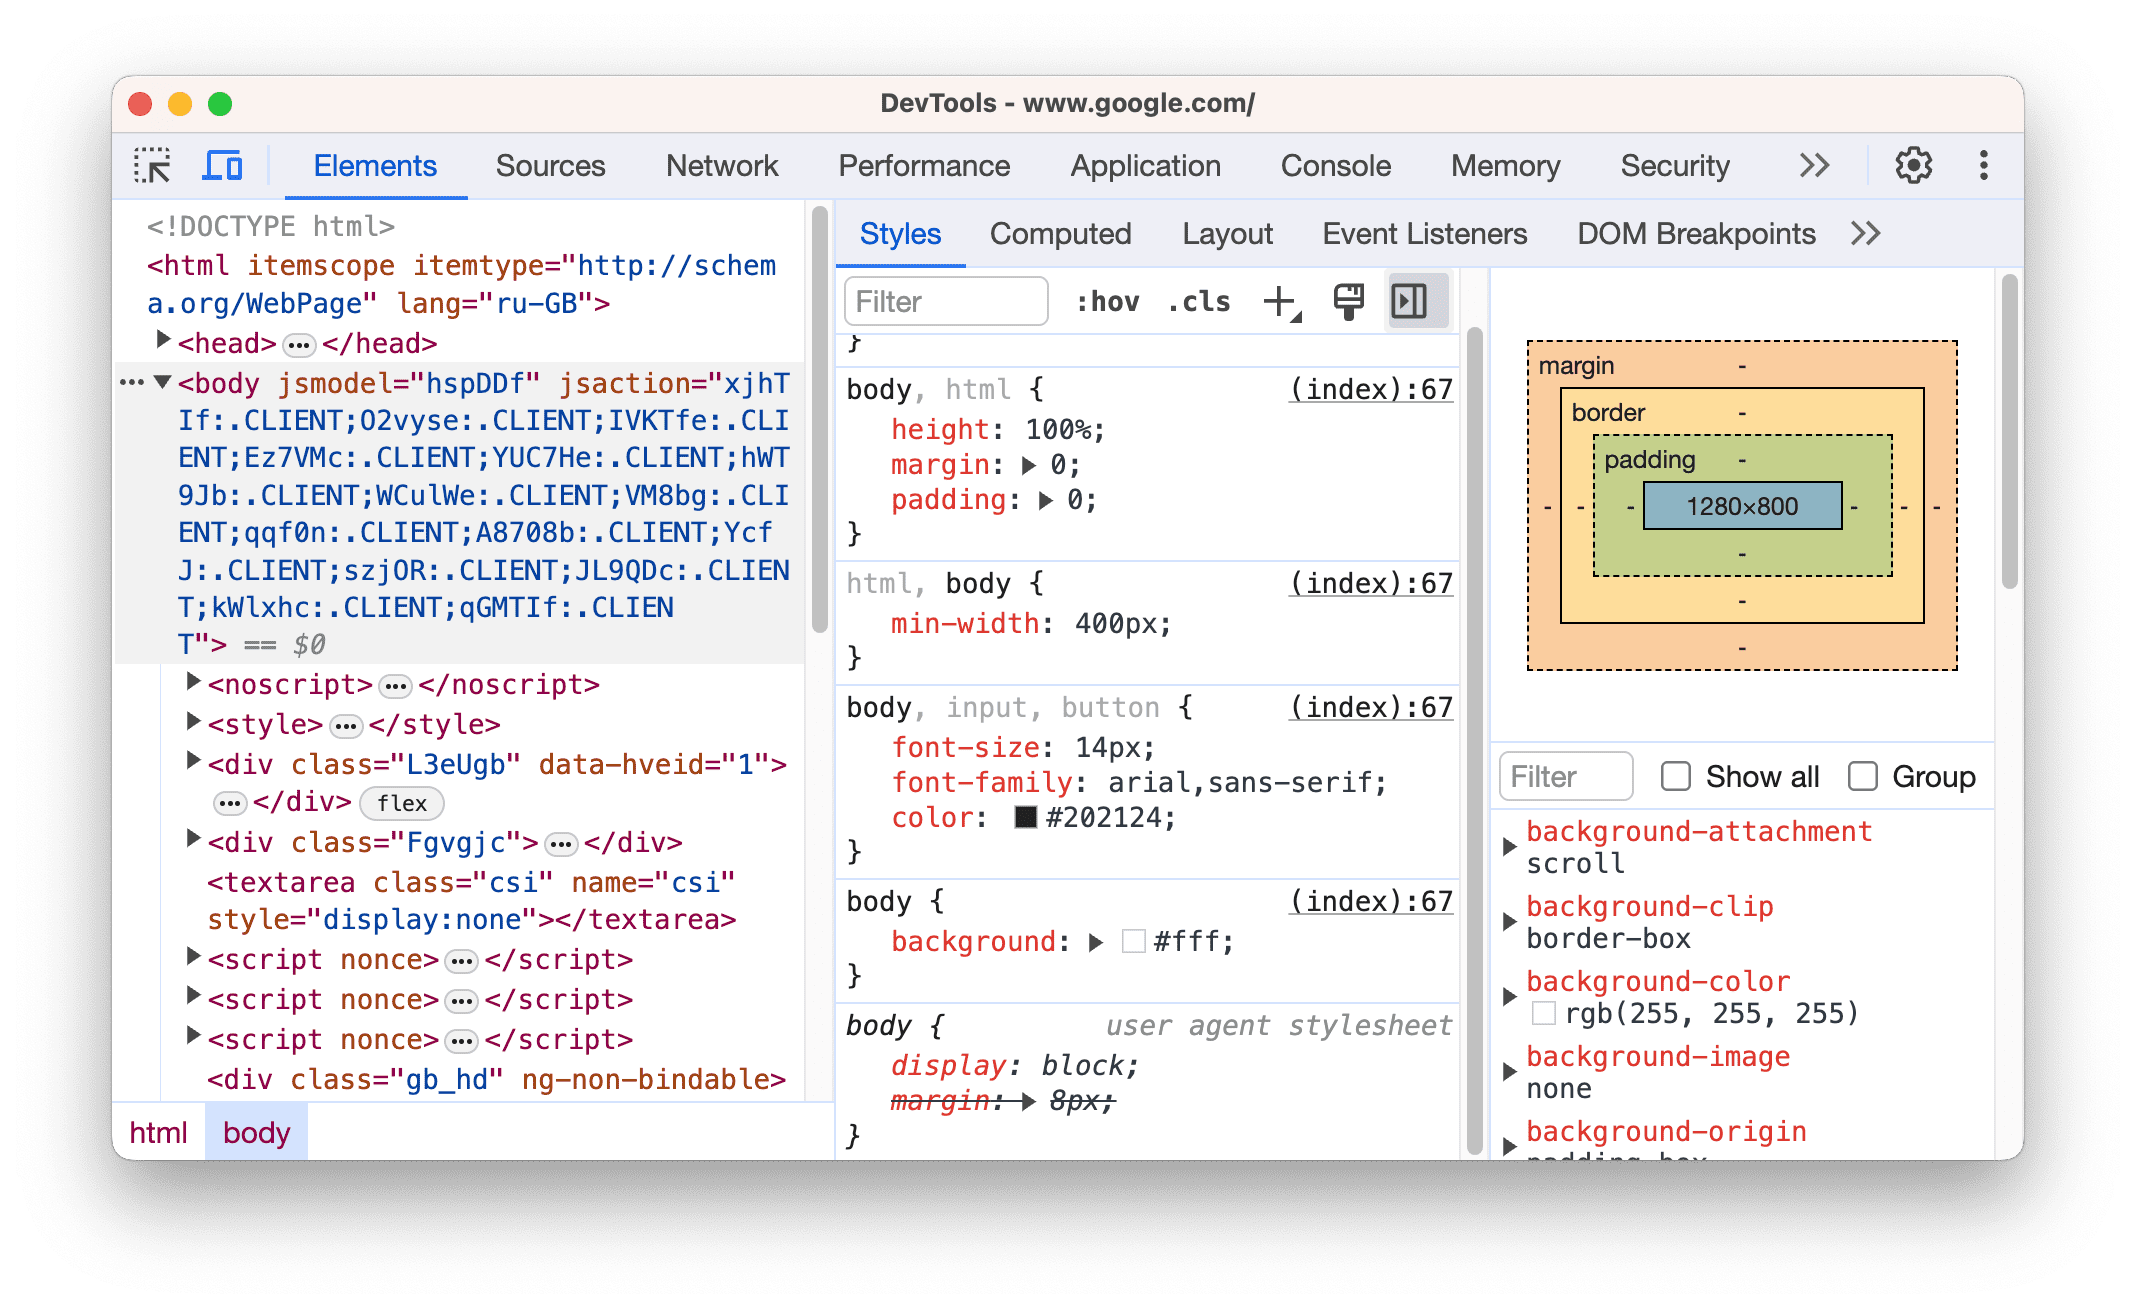
\includegraphics[width=0.65 \linewidth]{assets/chrome-devtools.png}\\
    {\footnotesize Fonte: Chrome for Developers}
    \label{fig:chrome-devtools}
\end{figure}
\newpage
\section{Firefox Developer Tools}
O Firefox Developer Tools, ilustrado na Figura \ref{fig:firefox}, oferece uma alternativa robusta aos Chrome DevTools, com um foco em privacidade e personalização. Essas ferramentas proporcionam um ambiente de desenvolvimento completo, permitindo a inspeção de elementos, a análise de redes, o depurador de JavaScript, a visualização de estilos CSS e a otimização do desempenho. Além disso, o Firefox Developer Tools se integra perfeitamente com outras ferramentas do ecossistema Mozilla, como o editor de código Visual Studio Code, facilitando o fluxo de trabalho dos desenvolvedores \cite{firefox}.
\begin{figure}[!htb]
    \centering
    \caption{Firefox Developer Tools}
    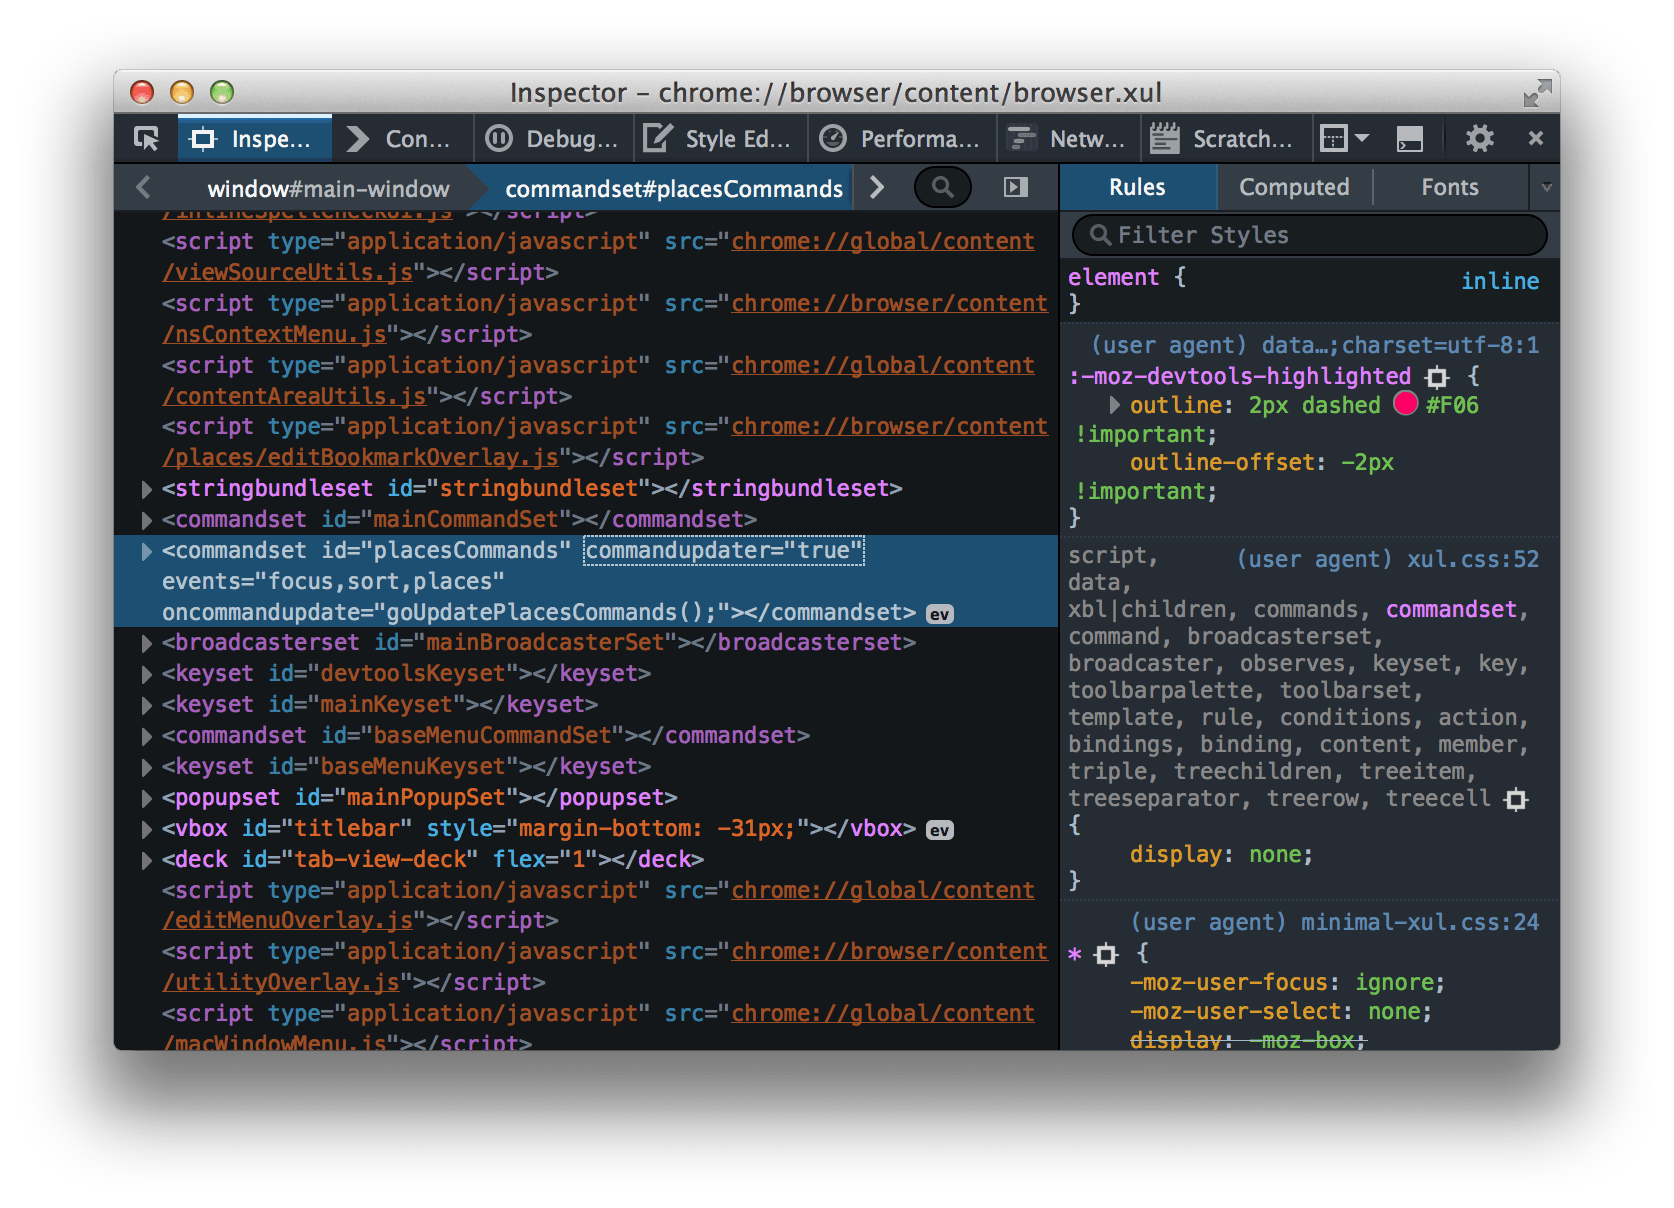
\includegraphics[width=0.8\linewidth]{assets/firefox.png}\\
    {\footnotesize Fonte: Firefox Source Tree Documentation}
    \label{fig:firefox}
\end{figure}
\section{Edge DevTools}
Os Edge DevTools, ilustrado na Figura \ref{fig:edge}, incorporados ao navegador Microsoft Edge, oferecem uma experiência de desenvolvimento moderna e eficiente. Com uma interface visualmente atraente e funcionalidades similares aos Chrome DevTools, os Edge DevTools permitem inspecionar elementos, depurar JavaScript, analisar o desempenho da página e simular diferentes dispositivos. A integração com o Microsoft Visual Studio Code e outras ferramentas do ecossistema Microsoft torna os Edge DevTools uma opção atraente para desenvolvedores que utilizam a plataforma Windows\cite{edge}.

\begin{figure}[!htb]
    \centering
    \caption{Edge DevTools}
    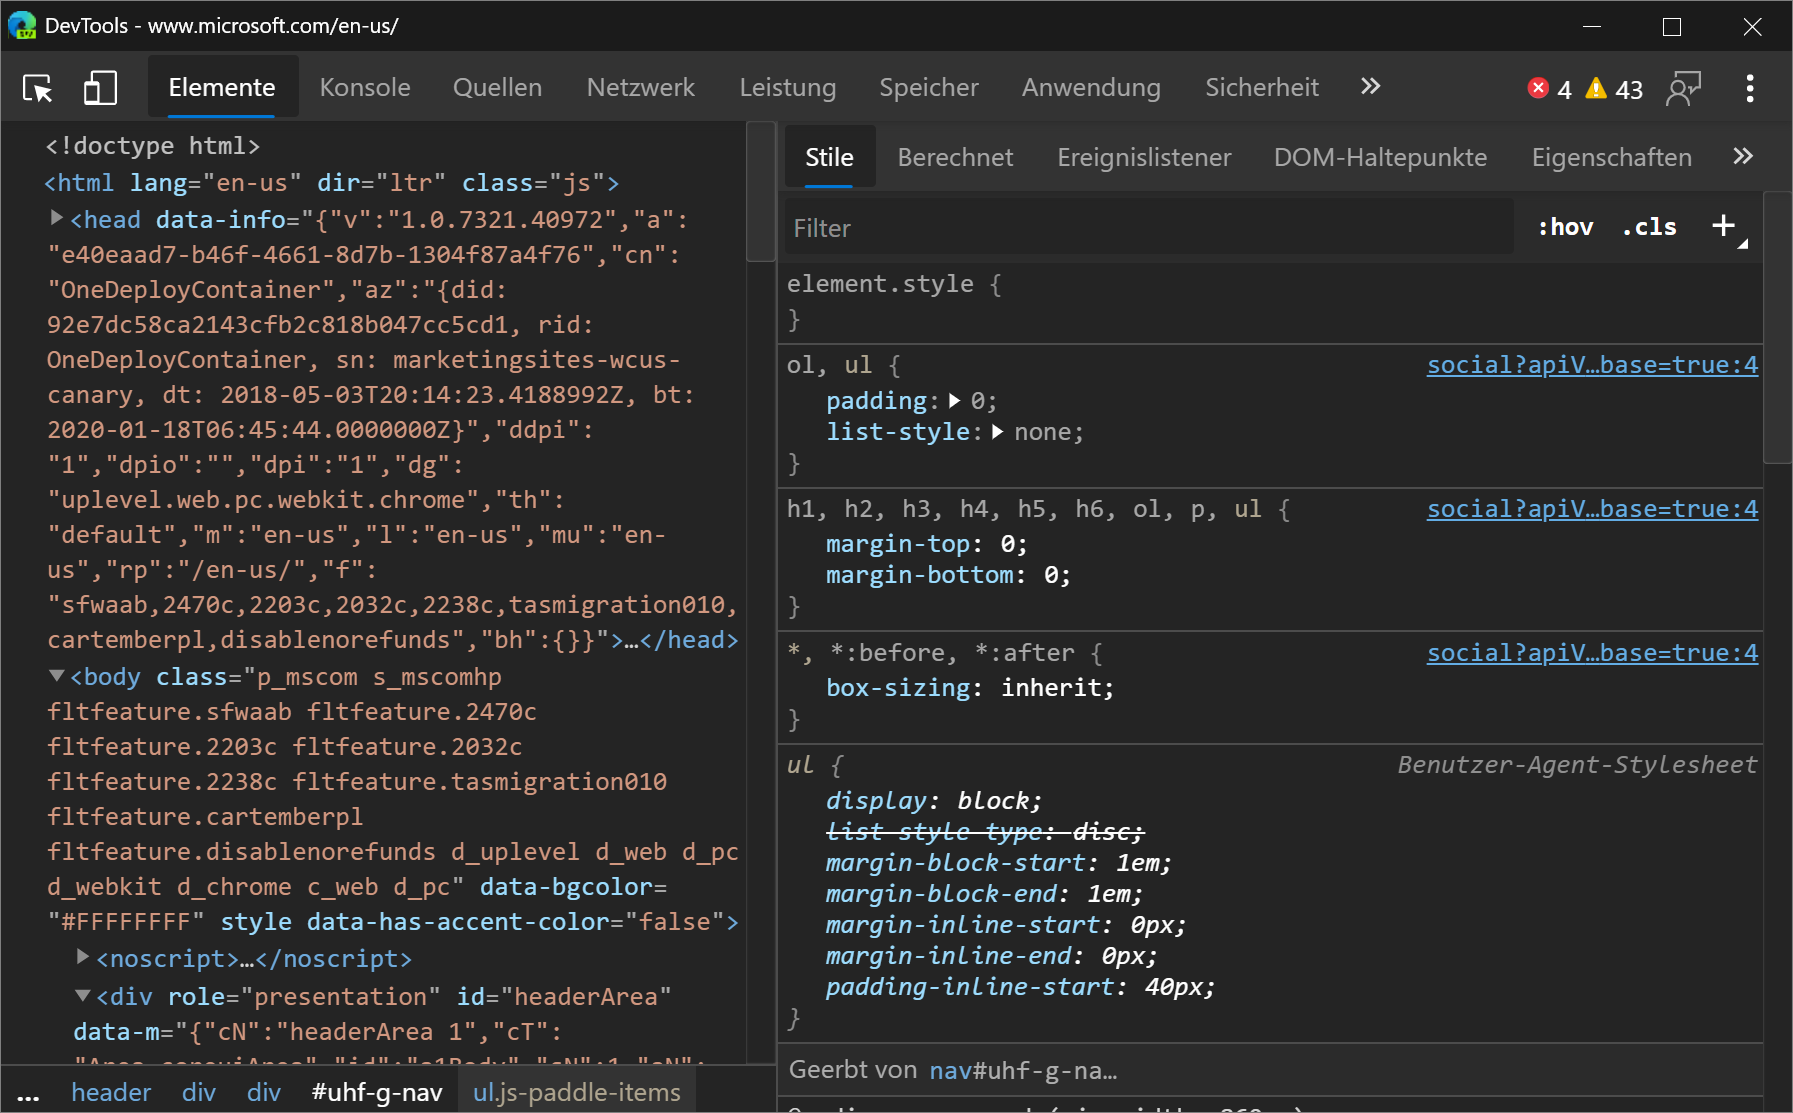
\includegraphics[width=0.8\linewidth]{assets/edge.png}\\
    {\footnotesize Fonte: Microsoft Learn}
    \label{fig:edge}
\end{figure}
\section{Safari Web Inspector}
O Safari Web Inspector, ilustrado na Figura \ref{fig:safari}, é a ferramenta de desenvolvimento integrada ao navegador Apple Safari, projetada para oferecer uma experiência de depuração e desenvolvimento de alta qualidade. Com um foco em desempenho e usabilidade, o Web Inspector permite inspecionar elementos, depurar JavaScript, analisar o desempenho da página e simular diferentes dispositivos\cite{apple}.
\begin{figure}[!htb]
    \centering
    \caption{Safari Web Inspector}
    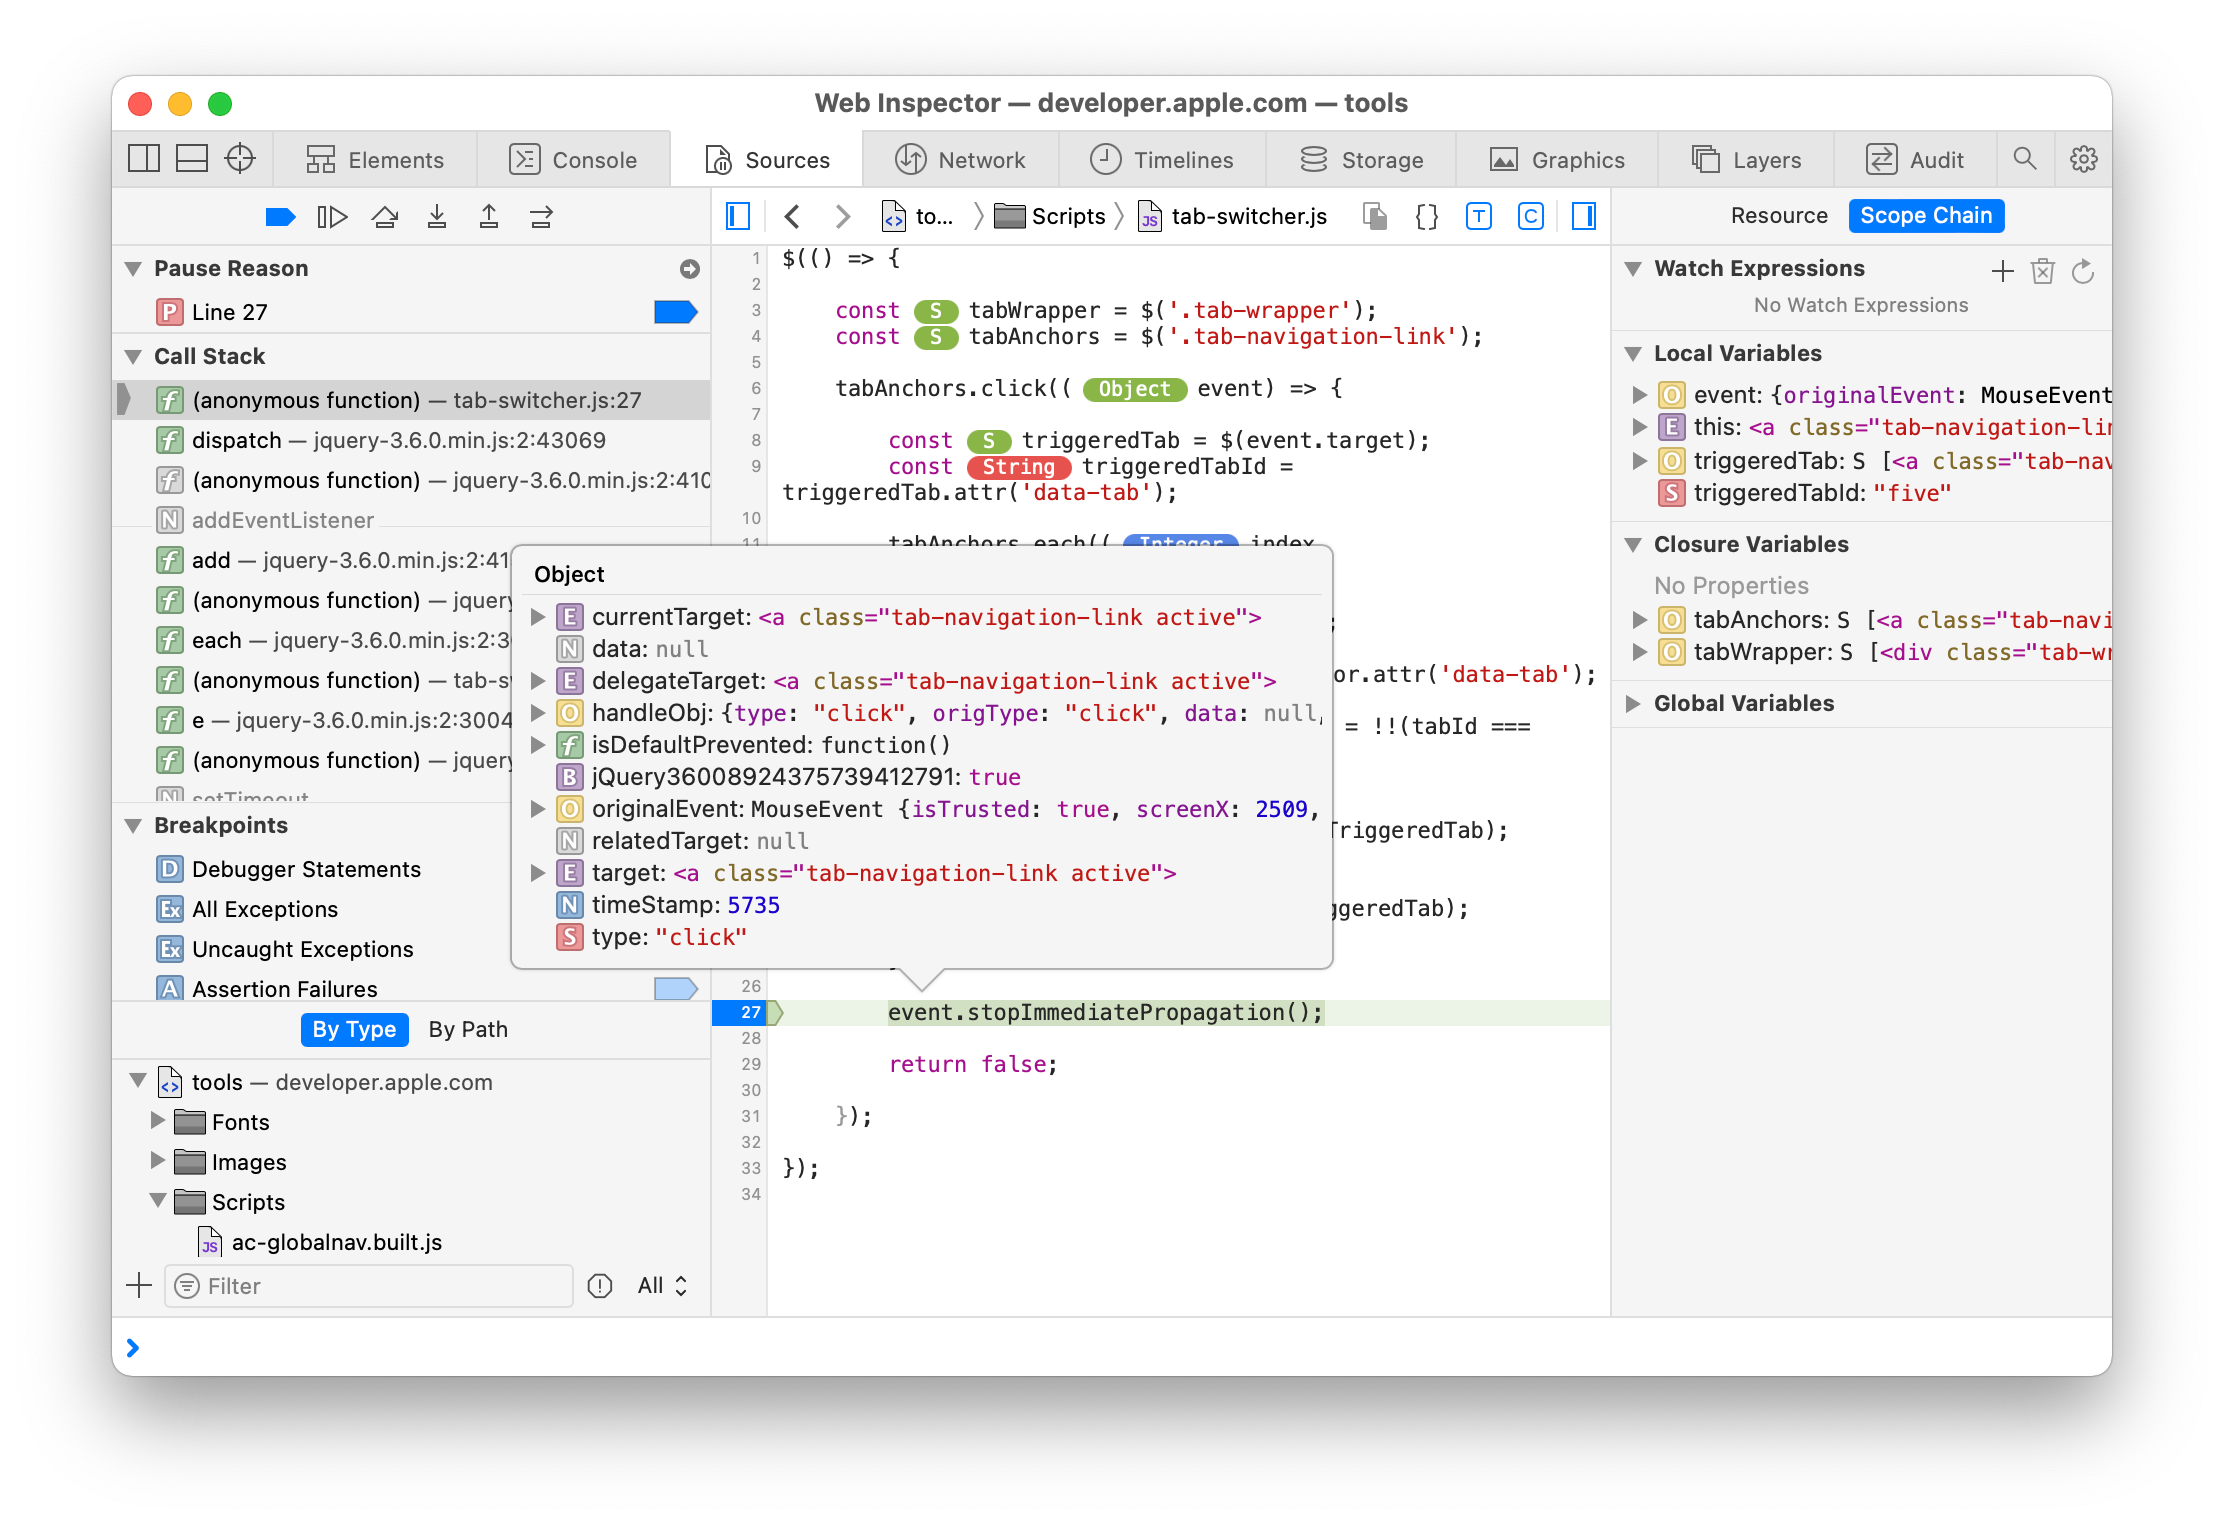
\includegraphics[width=0.8\linewidth]{assets/safari.png}\\
    {\footnotesize Fonte: Apple Developer Documentation}
    \label{fig:safari}
\end{figure}
\chapter{Metodologia}
\label{chap:metodologia}

Para o desenvolvimento deste trabalho optou-se por uma abordagem de análise exploratória. Este método se mostra especialmente adequada para este tema. Este método permite um exame detalhado e flexível do tema, proporcionando analises valiosas sobre as funcionalidades e características das ferramentas investigadas, bem como suas aplicações práticas no contexto do desenvolvimento web.

O campo é caracterizado por um rápido avanço tecnológico e pela ampla diversidade de soluções disponíveis. Assim, uma análise exploratória permite identificar padrões, relações e tendências que não seriam facilmente percebidos por meio de abordagens mais restritivas ou estruturadas.

\section{Analise exploratória}
A análise exploratória é uma metodologia qualitativa que busca compreender fenômenos, identificar tendências e levantar hipóteses a partir de dados ou informações iniciais \cite{analise-exploratoria}. Em contraste com métodos estruturados, que partem de hipóteses previamente definidas, a análise exploratória permite maior flexibilidade e adaptação durante o processo, sendo amplamente utilizada em pesquisas iniciais ou contextos pouco conhecidos.

No contexto deste estudo, a análise exploratória se justifica por permitir uma investigação aberta das ferramentas de desenvolvimento web, explorando desde as funcionalidades nativas até extensões e práticas comuns entre desenvolvedores. Com isso, essa metodologia será utilizada para:

\begin{itemize}
    \item \textbf{Analisar as características das ferramentas}: comparar as funcionalidades, linguagens suportadas, comunidades e ecossistemas de cada ferramenta.
    \item \textbf{Identificar tendências}: observar a evolução das ferramentas ao longo do tempo, a emergência de novas tecnologias e a obsolescência de outras
    \item \textbf{Avaliar a percepção dos desenvolvedores}: por meio de pesquisas, compreender as preferências, necessidades e desafios dos desenvolvedores na escolha de ferramentas.
\end{itemize}

A aplicação dessa metodologia é realizada em etapas sequenciais, que envolvem desde a coleta de dados até a interpretação dos resultados obtidos.

\chapter{Pesquisa de campo}
Entre janeiro e abril de 2025, foi conduzida uma pesquisa de campo para compreender a percepção dos desenvolvedores de software sobre as \textit{devtools}, explorando suas preferências, usos no cotidiano e impactos em diferentes contextos e níveis de experiência. O objetivo foi identificar as funcionalidades mais valorizadas, os desafios enfrentados e a eficiência dessas ferramentas no fluxo de trabalho dos profissionais.

A pesquisa utilizou um formulário estruturado, aplicado por meio de uma plataforma digital, para coletar dados de um público amplo e diversificado. O formulário incluiu questões específicas para filtrar respostas, garantindo que apenas desenvolvedores fossem considerados, excluindo participantes fora do perfil, como não desenvolvedores web, o que assegurou a confiabilidade e validade dos resultados.

Ao todo, foram obtidas um total de 80 respostas, com participantes de diferentes estados brasileiros e diferentes níveis de experiência. Após a aplicação dos critérios de seleção, que filtraram os participantes para incluir apenas desenvolvedores web, 45 respostas foram selecionadas para análise, garantindo a relevância e a confiabilidade dos dados utilizados no estudo. 

\section{Resultados obtidos}
Os resultados revelam que as ferramentas de desenvolvimento são essenciais para o desenvolvimento front-end, sendo o Google Chrome o navegador dominante e a inspeção de elementos e o console os recursos mais utilizados. Embora muitos desenvolvedores considerem as DevTools suficientes, especialmente em níveis júnior e intermediário, desenvolvedores seniores frequentemente as complementam com ferramentas ou plugins de IDE, indicando que a complexidade do projeto influencia as preferências de ferramentas. 

Um fato interessante é que apenas 27\% dos desenvolvedores sabiam que o \textit{Chrome DevTools} oferece mais de 20 ferramentas, apesar de 67\% usarem o \textit{DevTools} diariamente. Isso sugere uma lacuna no conhecimento de todos os recursos oferecidos, especialmente entre desenvolvedores juniores e intermediários, que frequentemente utilizam um conjunto limitado de ferramentas, como inspeção de elementos e console.

A dificuldade moderada percebida por desenvolvedores juniores e sua dependência de recursos externos, como tutoriais e colegas, ressaltam a necessidade de melhores recursos educacionais para preencher a lacuna de conhecimento. Essas percepções sugerem que, embora essas ferramentas sejam valiosas, o aumento da divulgação e a oferta de guias e treinamento sobre seus recursos completos podem aprimorar sua eficácia no desenvolvimento web.
\chapter{Ferramentas disponibilizadas pelos navegadores}
Para compreender melhor as possibilidades oferecidas pelas DevTools e como elas podem ser otimizadas, esta seção apresenta uma lista das ferramentas disponíveis nos principais navegadores do mercado atualmente, explorando suas funcionalidades, onde estão disponíveis e aplicações práticas no desenvolvimento web. A lista será apresentada em ordem alfabética.

\section{Acessibilidade}

\begin{figure}[h!]
    \centering
    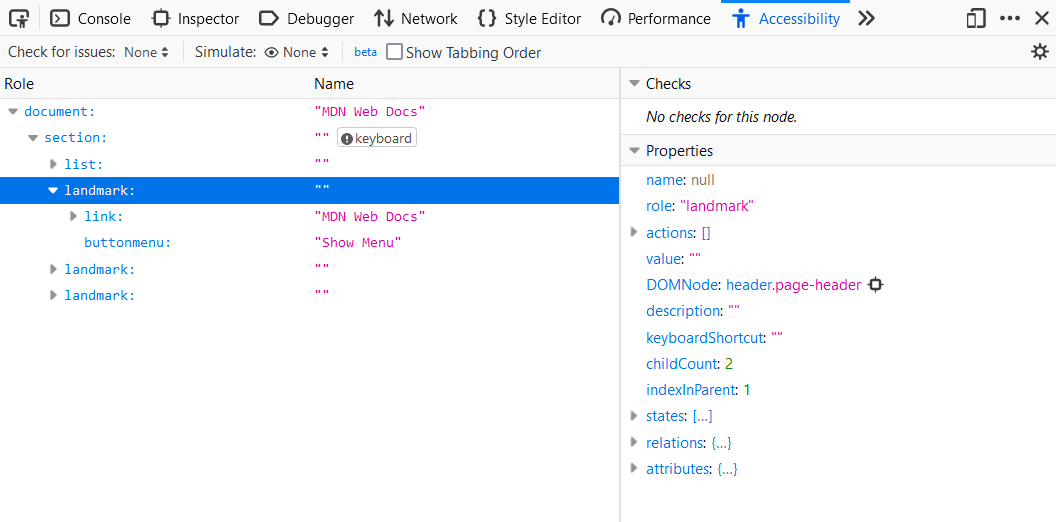
\includegraphics[width=0.7\linewidth]{assets/tools/firefox_accessibility.png}
    \caption{Aba de acessibilidade - Mozilla firefox}
    \label{fig:enter-label}
\end{figure}

As ferramentas de acessibilidade integradas nos navegadores modernos são fundamentais para desenvolvedores web, pois permitem a inspeção e a depuração de como as páginas interagem com as tecnologias assistivas. Essas ferramentas auxiliam na garantia de que o conteúdo web seja acessível a todos os usuários, independentemente de suas capacidades, tornando a experiência de navegação mais inclusiva \cite{firefox}.

No Chrome DevTools, o Lighthouse realiza auditorias abrangentes que incluem a avaliação da acessibilidade de um site, fornecendo relatórios e dicas para melhorias \cite{chrome}. As Ferramentas de Desenvolvedor do Firefox oferecem um "Accessibility inspector" que fornece acesso à árvore de acessibilidade da página, permitindo verificar o que está faltando ou precisa de atenção \cite{firefox}. O Web Inspector do Safari, por sua vez, na guia "Audit", contém auditorias que verificam as melhores práticas de acessibilidade do DOM, seguindo a especificação WAI-ARIA, como garantir que as tags de imagem tenham atributos \texttt{title} ou \texttt{alt} \cite{apple}. 
\newpage
\begin{lstlisting}[language=HTML, caption="Exemplo de imagem e correção sugerida"]
    <!-- incorreto -->
    <img src="exemplo.jpg" -->

    <!-- Correcao sugerida -->
    <img src="exemplo.jpg" alt="Descricao da imagem">
\end{lstlisting}


O Safari também oferece métodos para interagir com a árvore de acessibilidade, como \texttt{getElementsByComputedRole} e \texttt{getComputedProperties}, que retornam informações detalhadas sobre papéis e propriedades calculadas \cite{apple}.

\section{Alterações}
\begin{figure}[h!]
    \centering
    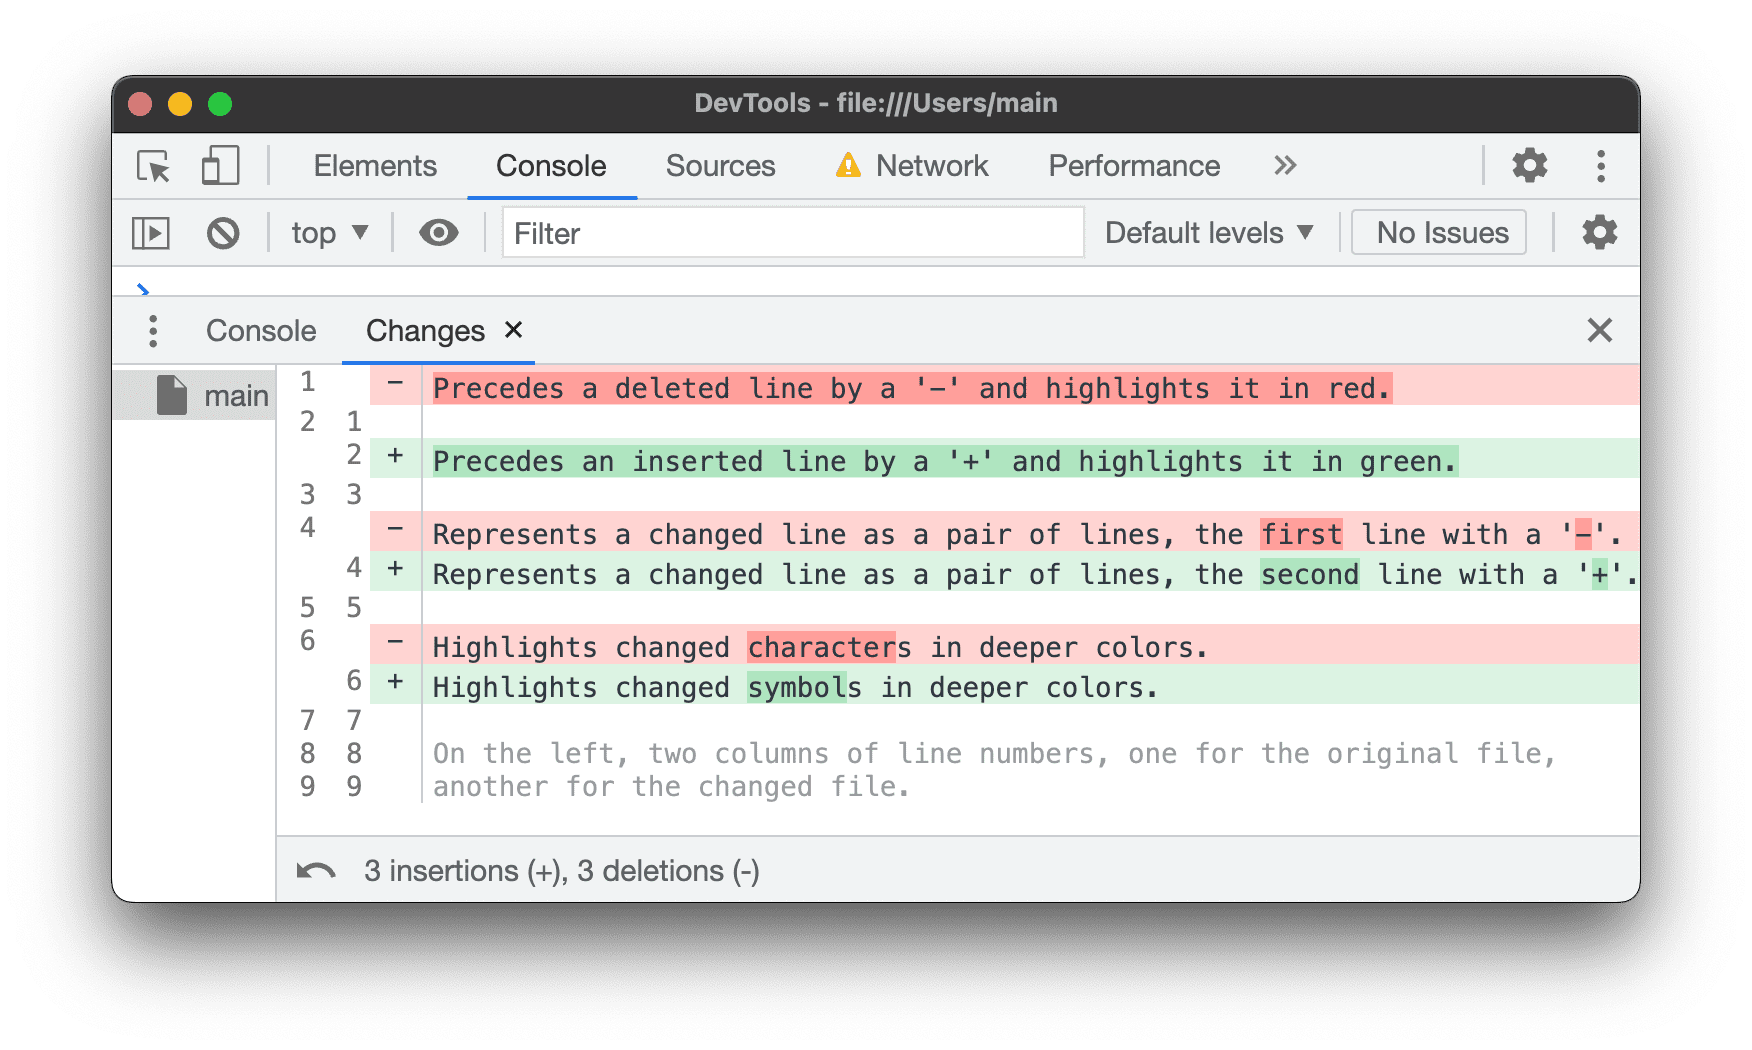
\includegraphics[width=0.7\linewidth]{assets/tools/changes-chrome.png}
    \caption{Aba de alterações - Google Chrome}
    \label{fig:enter-label}
\end{figure}
O painel Changes (Alterações) no Chrome DevTools é uma ferramenta que permite aos desenvolvedores acompanhar as modificações de código feitas diretamente dentro do DevTools. Ele rastreia as alterações em HTML (quando as substituições locais estão ativadas no painel Fontes), CSS (tanto no painel Elementos > Estilos quanto no Fontes) e JavaScript (no painel Fontes). O objetivo principal é fornecer uma visão clara do que foi modificado durante uma sessão de depuração ou experimentação \cite{chrome}.

É importante notar que as alterações registradas pelo painel Changes não são permanentes e serão perdidas ao recarregar a página ou fechar o DevTools, a menos que sejam salvas explicitamente usando substituições locais ou configurando um espaço de trabalho \cite{chrome}. Essa característica contrasta fundamentalmente com o Git, um sistema de controle de versão distribuído, onde todas as modificações são registradas de forma permanente e rastreável em um histórico \cite{git}. 

O painel apresenta uma saída "diff" que destaca as adições e exclusões no código. Além disso, oferece funcionalidades como copiar todas as alterações registradas pelo painel \cite{chrome}.

\section{Animações}
\begin{figure}[h!]
    \centering
    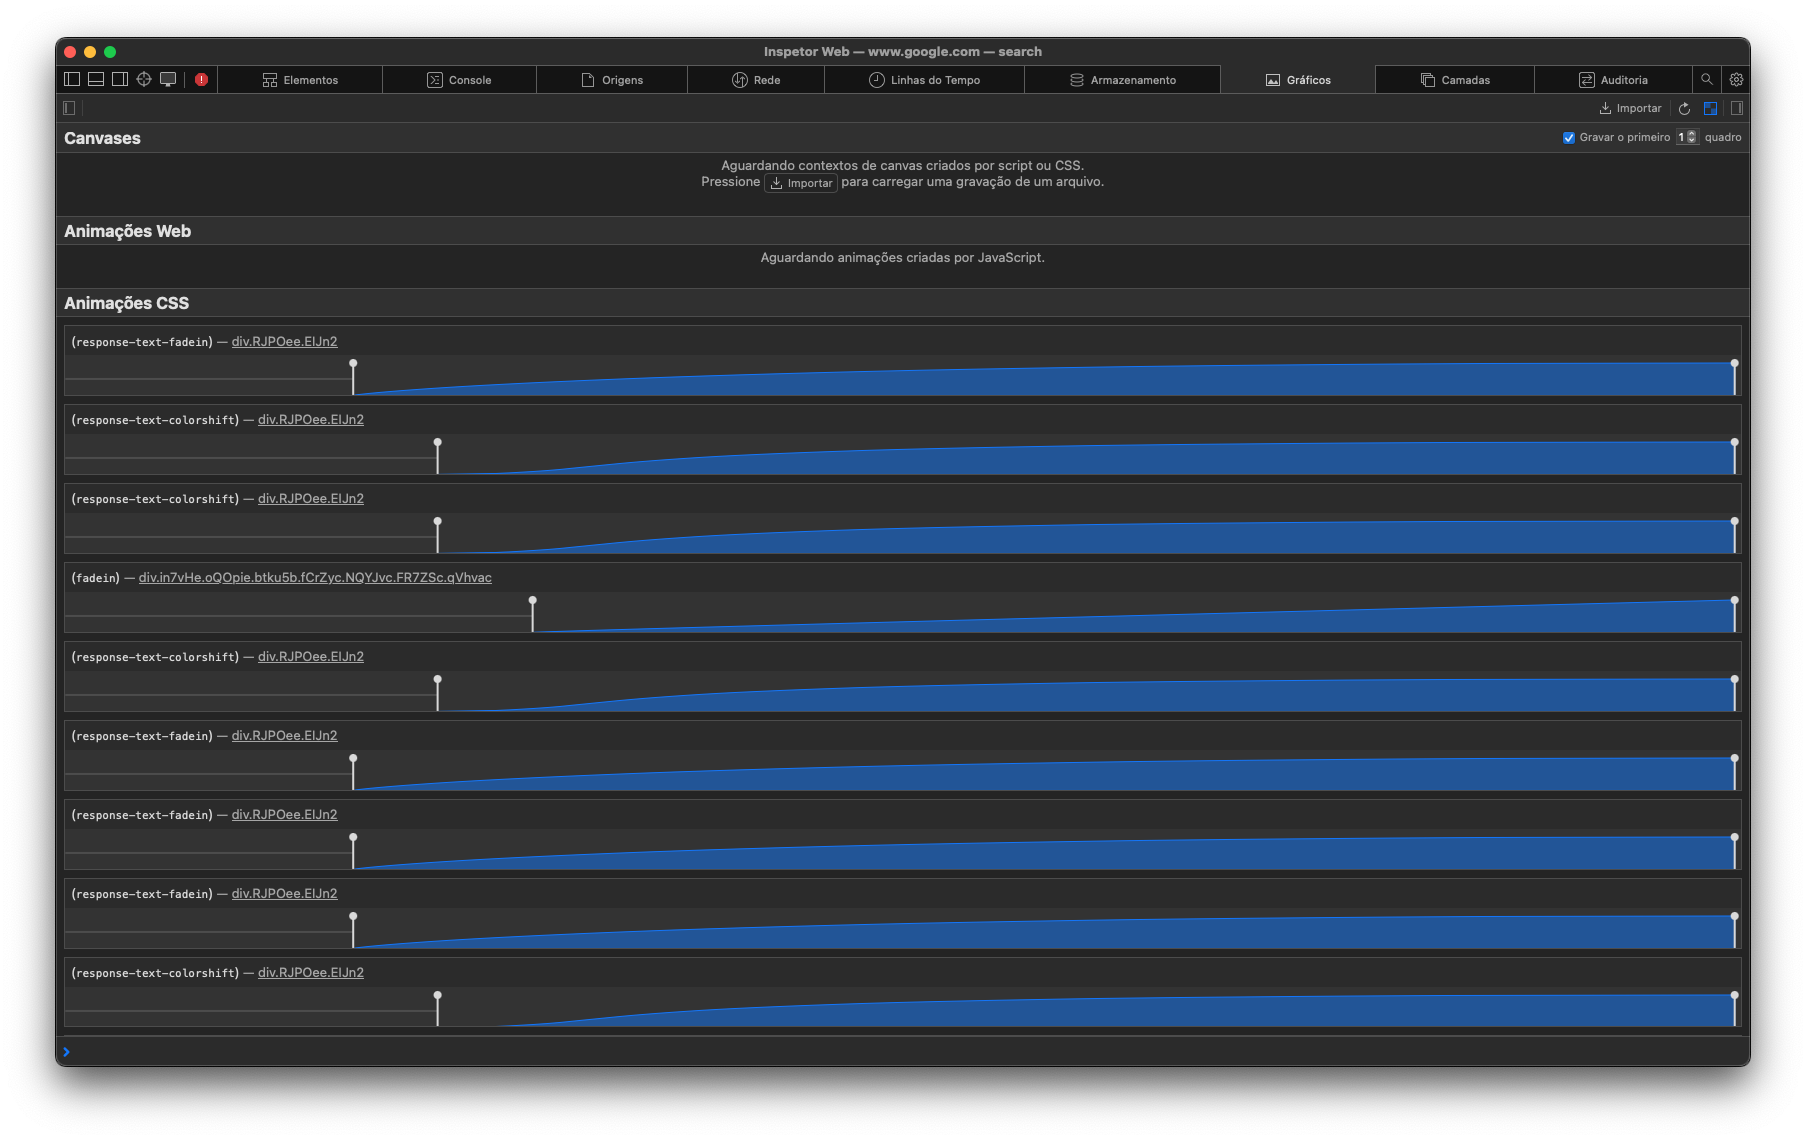
\includegraphics[width=0.7\linewidth]{assets/tools/safari-graficos.png}
    \caption{Aba de graficos - Safari }
    \label{fig:enter-label}
\end{figure}

As ferramentas de animação nos navegadores são projetadas para inspecionar e modificar animações em páginas web. Elas detectam automaticamente as animações e as organizam em grupos, permitindo visualizar seus detalhes, como definições e iterações, e identificar se várias animações estão aplicadas a elementos diferentes com a mesma cor \cite{chrome}. Essas ferramentas suportam animações CSS, transições CSS, animações Web e a API View Transitions. O Safari Web Inspector também oferece uma aba "Graphics" com "Animation Preview" para pré-visualizar keyframes e classes de animações, incluindo as de HTML5 canvas, JavaScript e CSS, para ajustar o movimento e o design visual \cite{apple}.

Para depuração e otimização, essas ferramentas permitem diminuir a velocidade, repetir ou inspecionar o código-fonte de um grupo de animação, além de modificar o tempo, o atraso, a duração ou os deslocamentos dos keyframes. A capacidade de editar \texttt{\@keyframes} em tempo real na seção "Estilos" e ver as mudanças refletidas imediatamente no painel "Animações" é um recurso valioso para ajuste fino \cite{chrome}. 

\section{Armazenamento}
As ferramentas de armazenamento nos navegadores, como as encontradas no Chrome DevTools, Edge Devtools, Firefox DevTools e Safari Web Inspector, são essenciais para inspecionar, modificar e depurar diversos aspectos relacionados à persistência de dados em aplicações web. Elas oferecem uma visão detalhada sobre como as páginas web armazenam informações no dispositivo do usuário, auxiliando os desenvolvedores a entender e gerenciar dados em tempo real.

\begin{figure}[h!]
    \centering
    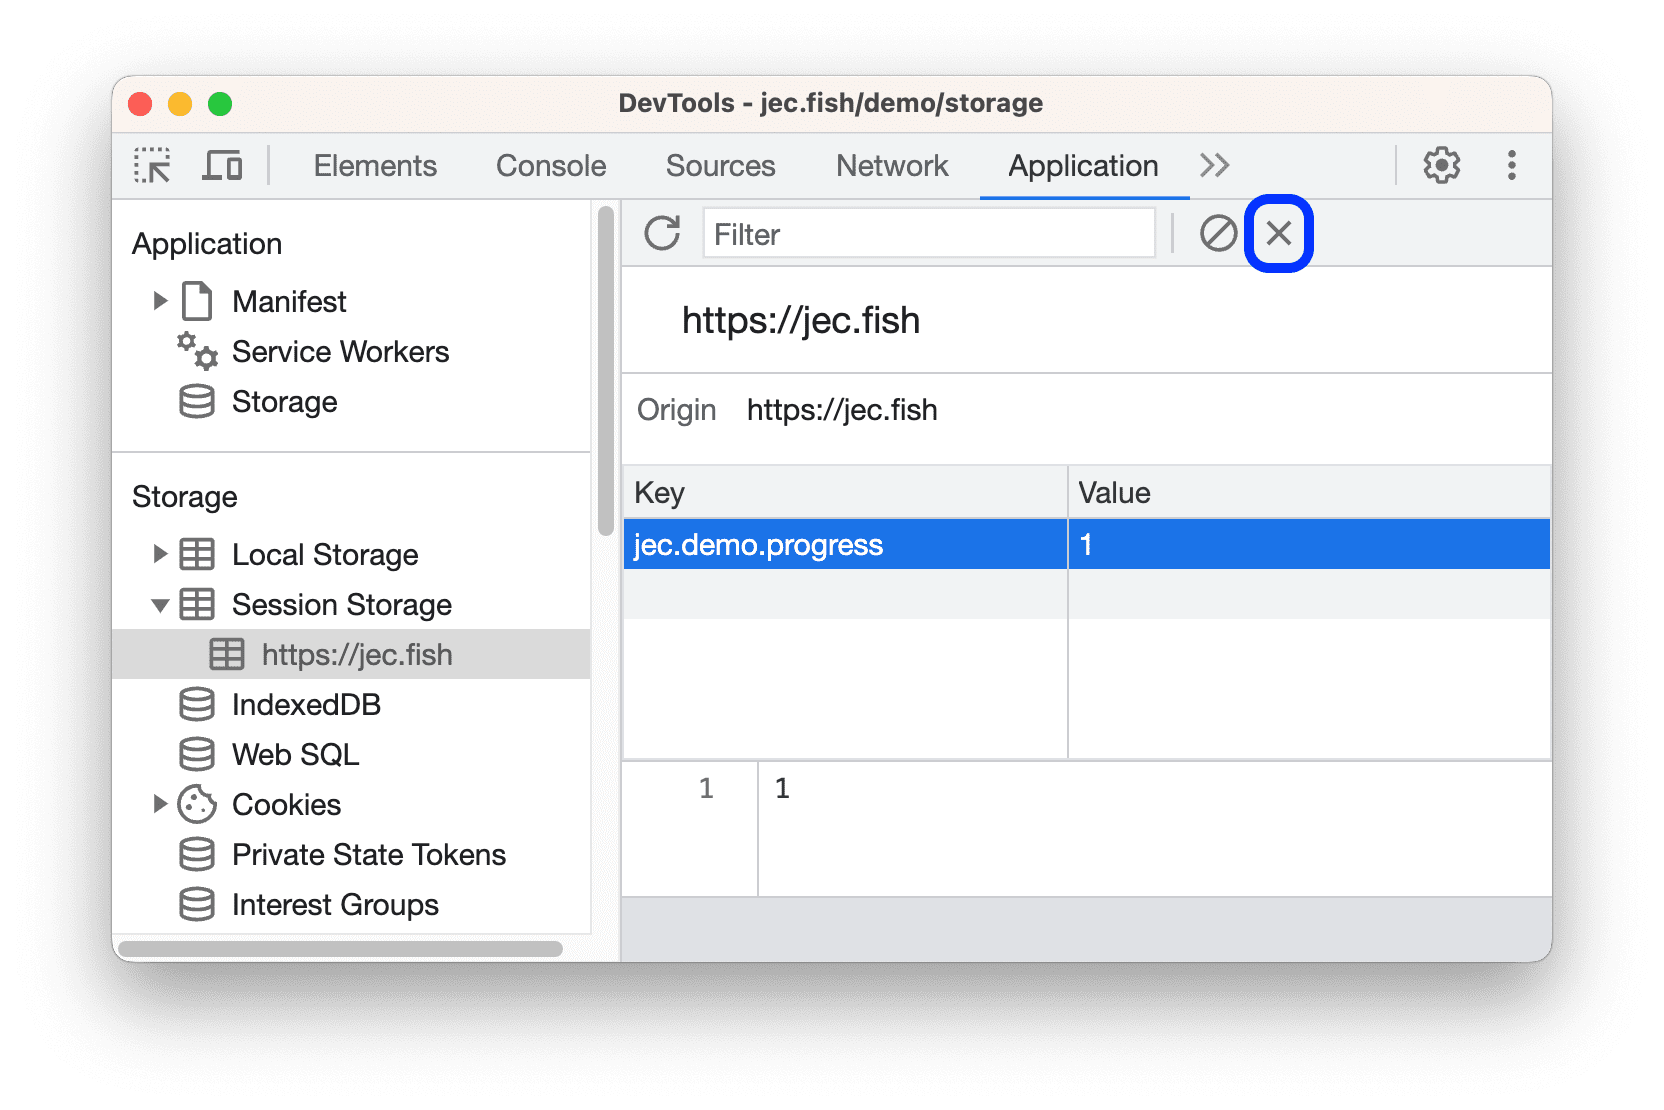
\includegraphics[width=0.7\linewidth]{assets/tools/chrome-storage.png}
    \caption{Aba de armazenamento - Google Chrome }
    \label{fig:enter-label}
\end{figure}

Essas ferramentas permitem a inspeção de vários tipos de armazenamento, incluindo cookies, armazenamento local (localStorage), armazenamento de sessão (sessionStorage), IndexedDB (bancos de dados indexados) e Cache Storage (caches de API) \cite{edge}.
Além de visualizar dados, os desenvolvedores podem editar pares de chave-valor para armazenamento local e de sessão, limpar cookies e excluir recursos em cache, o que é crucial para testar diferentes estados de usuário ou cenários de privacidade. O Safari Web Inspector também oferece controle sobre o cache de aplicação.

No geral, as ferramentas de armazenamento são fundamentais para depurar problemas de persistência de dados, como conteúdo obsoleto, valores incorretos ou problemas de quota de armazenamento \cite{apple}. Elas permitem verificar se os dados estão sendo armazenados e recuperados corretamente, limpar dados problemáticos para testar estados iniciais e simular diferentes cenários de armazenamento, contribuindo para o desenvolvimento de aplicações web robustas e confiáveis, especialmente aquelas que dependem de capacidades offline ou preferências de usuário persistentes.

\section{Autofill}
A ferramenta de autofill são uteis para auxiliar desenvolvedores a inspecionar e depurar informações de endereço salvas, otimizando a experiência de preenchimento de formulários em websites. Atualmente, somente o Chrome DevTools possui um painel Autofill dedicado a essa funcionalidade, que permite visualizar o mapeamento entre os campos do formulário, os valores de autofill previstos pelo navegador e os dados salvos \cite{chrome}.

\begin{figure}[h!]
    \centering
    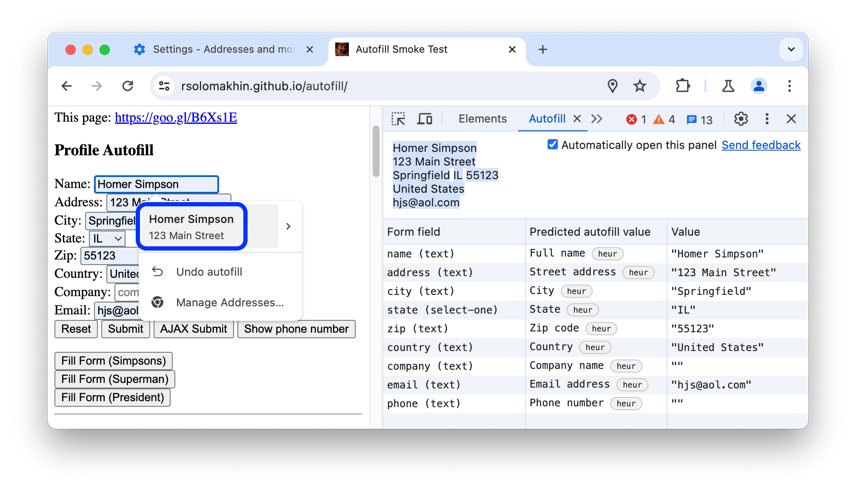
\includegraphics[width=0.7\linewidth]{assets/tools/chrome-autofill.png}
    \caption{Aba de autofill - Google Chrome }
    \label{fig:enter-label}
\end{figure}

O painel Autofill do Chrome pode ser aberto automaticamente ao preencher um formulário com as Ferramentas do Desenvolvedor abertas, ou manualmente através do menu de comando. Ao interagir com um formulário, o painel exibe uma tabela detalhada com os campos detectados, a previsão de preenchimento automático e os valores inseridos \cite{chrome}. É possível até mesmo usar dados de teste de endereço fornecidos pelo próprio painel para facilitar a depuração. Para problemas relacionados a atributos de autofill, o painel de Problemas também pode fornecer dicas de correção.

\section{Camadas}
\begin{figure}[h!]
    \centering
    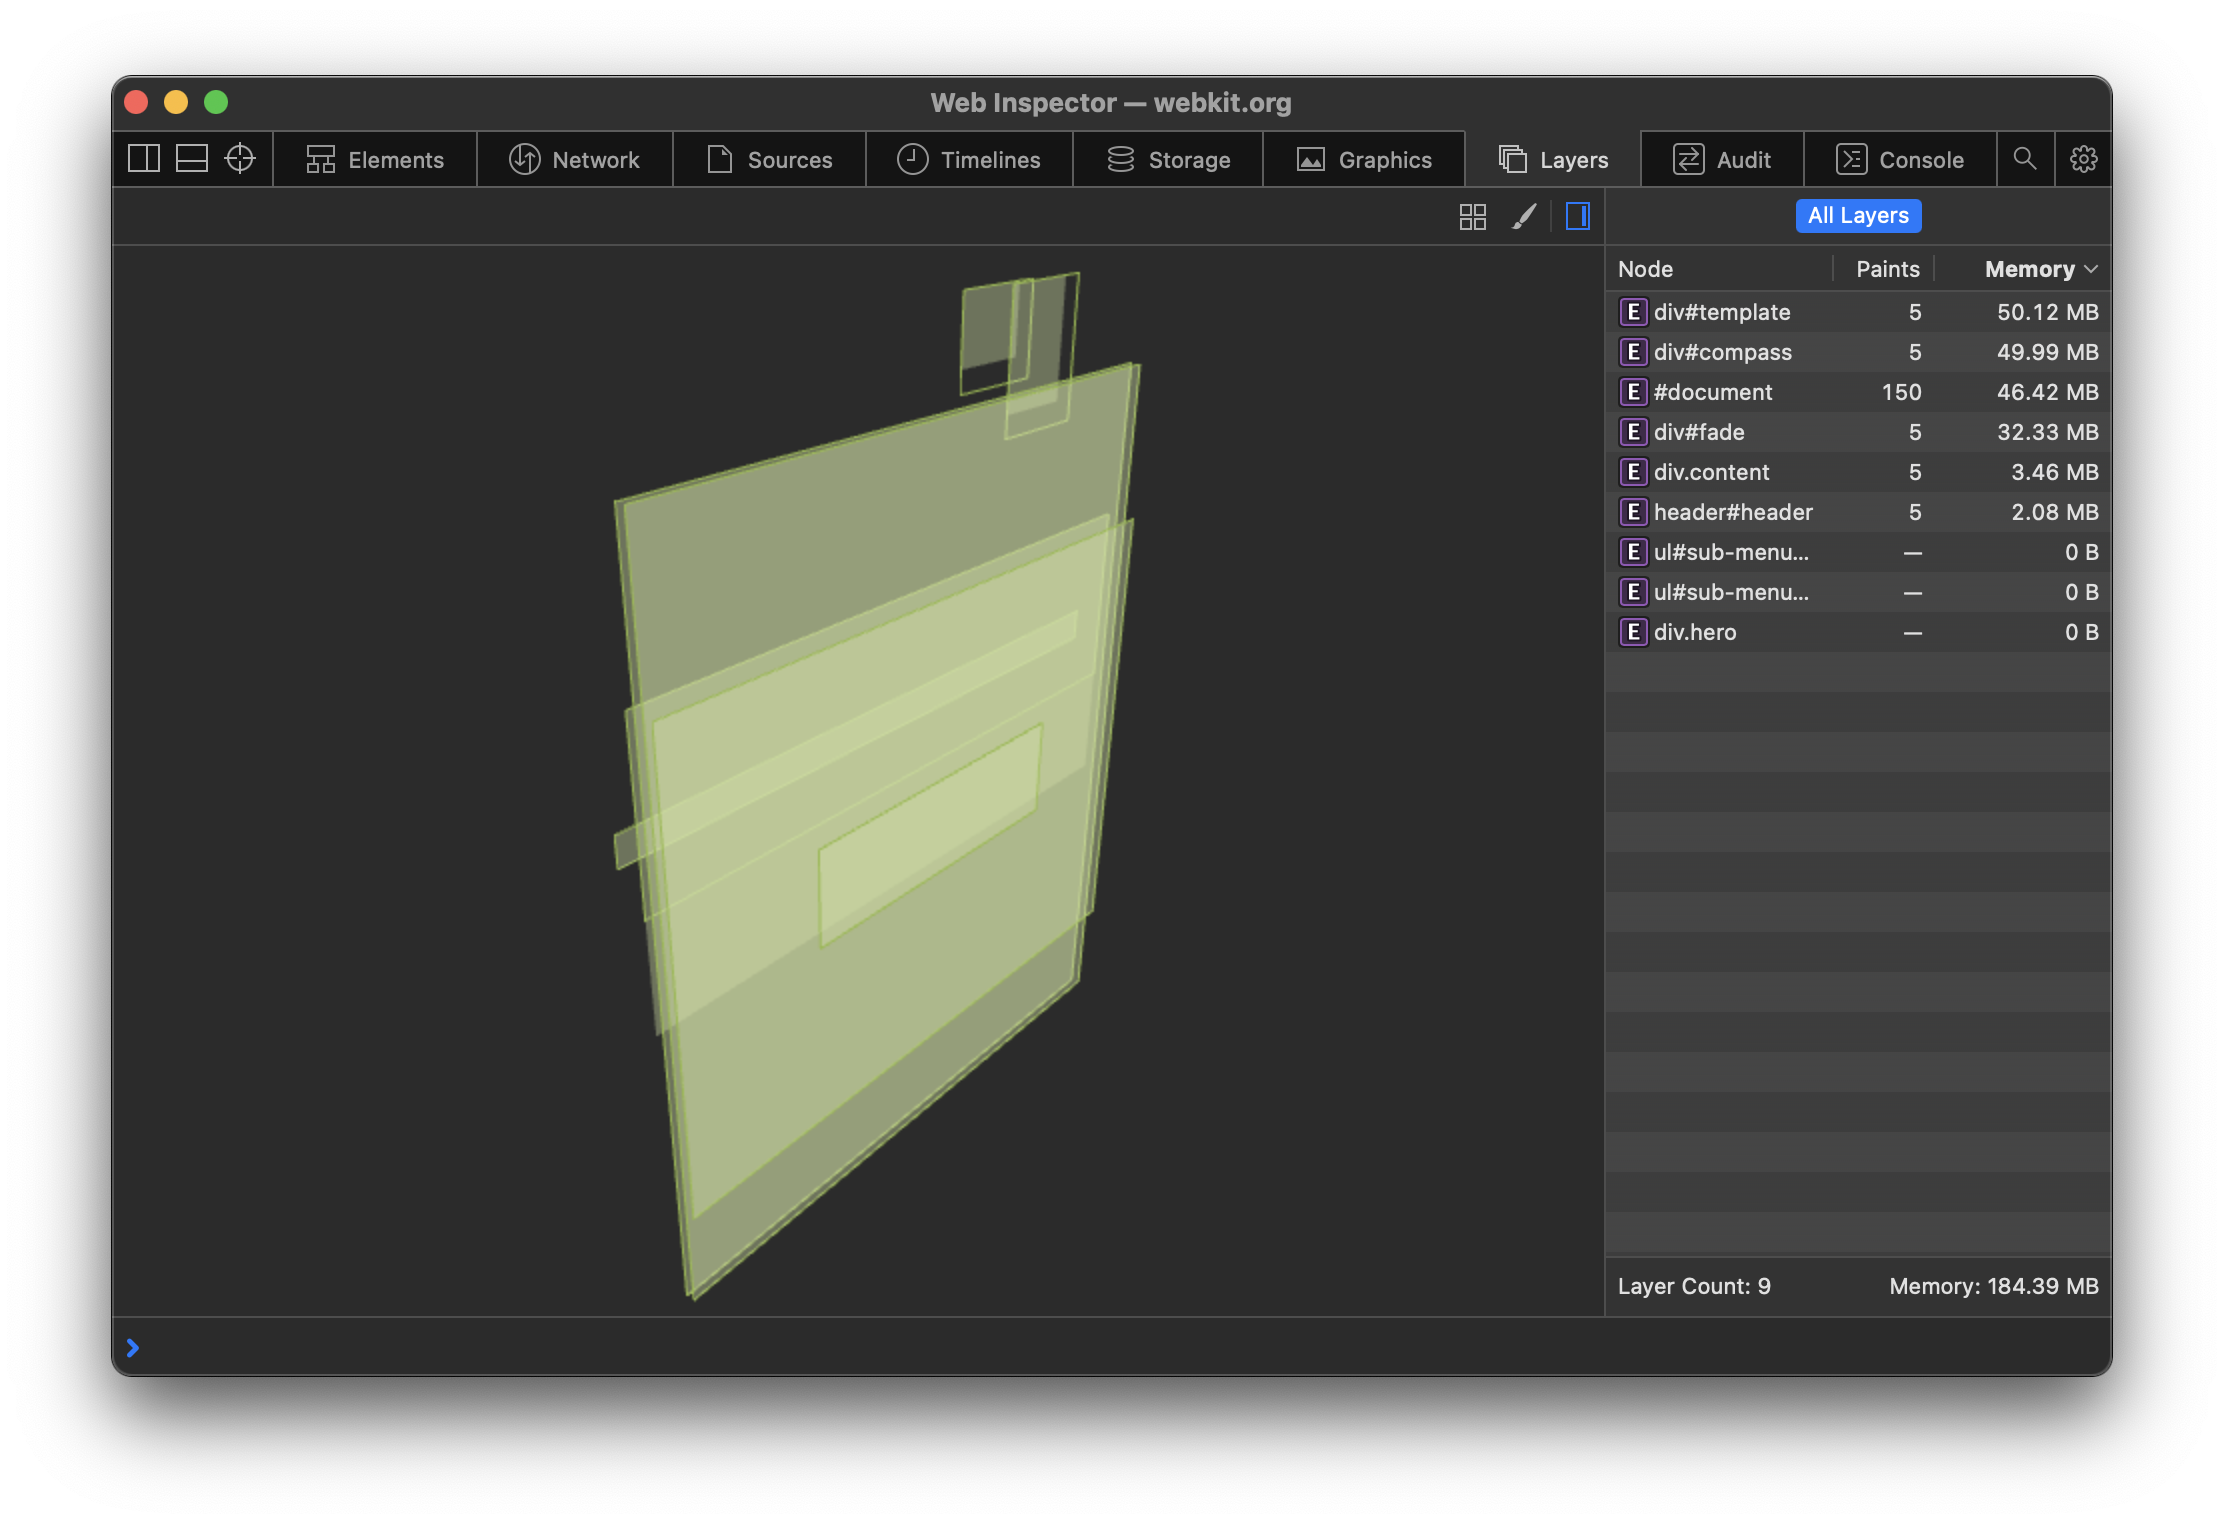
\includegraphics[width=0.7\linewidth]{assets/tools/safari-layers.png}
    \caption{Aba de camadas - Safari }
    \label{fig:enter-label}
\end{figure}
As ferramentas de desenvolvimento integradas nos navegadores modernos, como Chrome e Safari, oferecem funcionalidades para visualizar e analisar a composição de elementos de uma página web em camadas, muitas vezes em uma representação 3D \cite{apple, chrome}. Essas ferramentas auxiliam o desenvolvedor entender como o navegador renderiza o conteúdo, identificar gargalos de desempenho e depurar problemas relacionados à renderização e ao layout.

No Chrome DevTools, o painel "Layers" (Camadas) permite aos desenvolvedores visualizar as camadas de um documento em uma árvore expansível e um diagrama 3D. É possível inspecionar camadas para ver informações como tamanho, motivos para a composição, estimativa de memória, contagem de pintura e regiões de rolagem lenta. Além disso, o painel oferece recursos visuais, como o Paint Profiler e a capacidade de destacar regiões de rolagem lenta em rosa, ajudando a identificar elementos que podem prejudicar a performance \cite{chrome}. Similarmente, o Safari Web Inspector possui uma aba "Layers" que oferece uma visualização interativa em 3D da árvore de camadas da página inspecionada, mostrando informações básicas como contagem de pintura cumulativa e custo de memória, além dos motivos pelos quais uma camada foi criada \cite{apple}.
\section{Captura de tela}
\begin{figure}[h!]
    \centering
    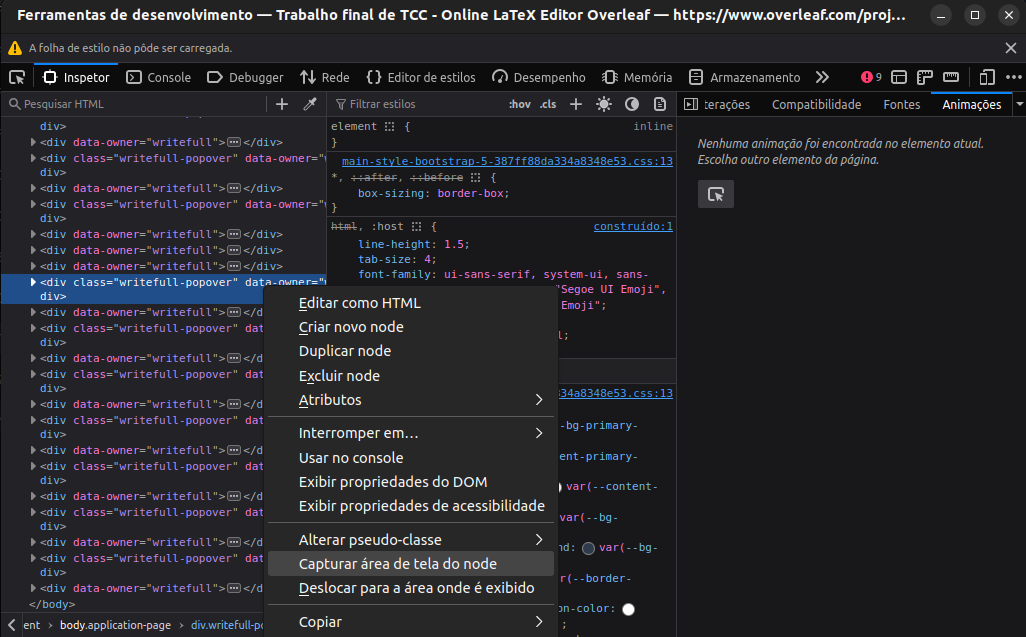
\includegraphics[width=0.7\linewidth]{assets/tools/firefox-screenshot.png}
    \caption{Opçao de captura de tela - Mozilla Firefox }
    \label{fig:enter-label}
\end{figure}
Durante o processo de desenvolvimento de sistemas web, uma ferramenta que auxilia na depuração e otimização visual da página web é a captura de tela, também conhecida pela sua tradução em inglês \textit{screenshot}. No Firefox, especificamente, a funcionalidade de captura de tela pode ser acessada de diversas maneiras. Uma opção é utilizar o ícone dedicado na barra de ferramentas para capturar a página completa \cite{firefox}. Alternativamente, é possível realizar a captura de um elemento HTML específico diretamente do Inspetor HTML, clicando com o botão direito do mouse sobre o elemento desejado e selecionando a opção "Screenshot Node" \cite{firefox}. Ambas as abordagens permitem copiar as imagens geradas diretamente para a área de transferência do sistema operacional.

É importante notar que, diferentemente do Firefox, os outros navegadores citados nesse trabalho não possuem um recurso de captura de tela autônomo diretamente acessível na barra de ferramentas. No entanto, essa funcionalidade essencial está integrada em suas respectivas ferramentas de desenvolvimento. Além disso, é importante reconhecer que a capacidade de captura de tela não se restringe aos navegadores web. Sistemas operacionais modernos, como Windows e macOS, já possuem essa ferramenta nativamente \cite{print-mac, print-windows}. Além disso, existem diferentes programas de terceiros, como o Lightshot, que são dedicados à captura de tela \cite{lightshot}. 

\section{Cobertura}
\begin{figure}[h!]
    \centering
    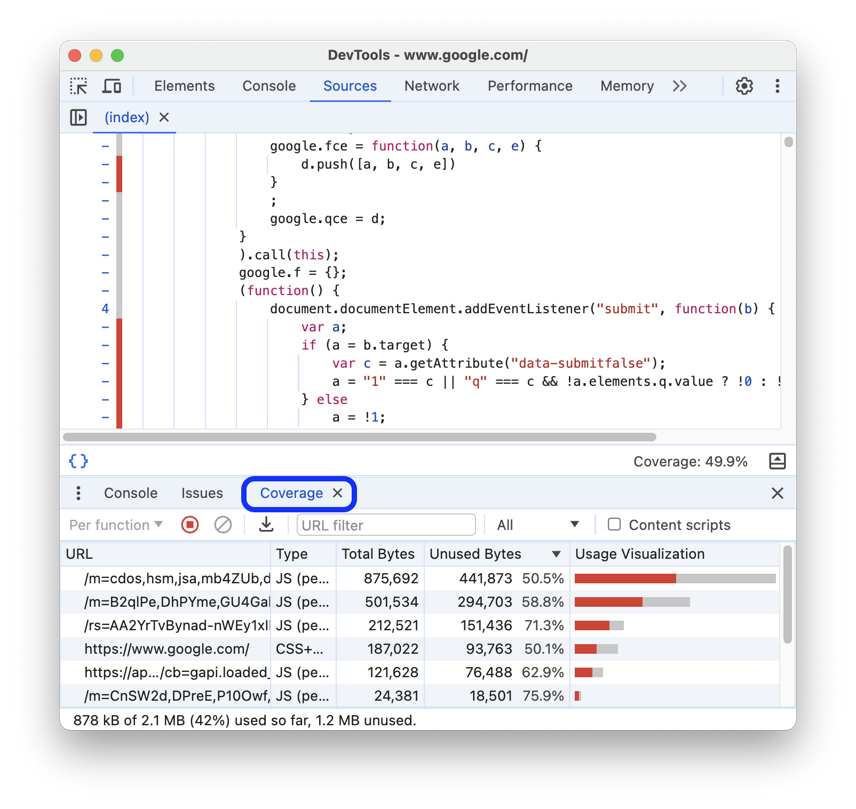
\includegraphics[width=0.7\linewidth]{assets/tools/chrome-coverage.png}
    \caption{Aba de cobertura de código - Google Chrome }
    \label{fig:enter-label}
\end{figure}
As ferramentas de cobertura de código integradas nos navegadores modernos auxiliam o desenvolvedor otimizar o desempenho de páginas web, permitindo identificar e eliminar código JavaScript e CSS não utilizado. No Google Chrome e no Microsoft Edge, o painel Coverage é a principal ferramenta para isso, fornecendo um relatório detalhado do total de bytes usados e não usados de recursos CSS e JavaScript \cite{chrome}. Ele visualiza esse código no painel Sources, marcando as linhas não executadas com barras vermelhas, o que ajuda a acelerar o carregamento da página e a economizar dados móveis dos usuários \cite{chrome}. Além disso, o painel permite escolher o escopo da análise (por função ou por bloco) e exportar o relatório para análises posteriores. Outros navegadores citados não possuem essa ferramenta de modo dedicado, apenas integrado com outras ferramentas.

Além das ferramentas de cobertura de código integradas aos navegadores, existem soluções dedicadas que oferecem funcionalidades mais abrangentes para a análise de código e testes automatizados. Plataformas como Cypress são amplamente utilizadas para testar a cobertura de código em ambientes de desenvolvimento e produção. O Cypress, por exemplo, é um framework de testes de ponta a ponta que pode ser configurado para gerar relatórios de cobertura de código detalhados, indicando quais partes da aplicação são exercitadas pelos testes \cite{cypress}. 

\section{Código fonte}
\begin{figure}[h!]
    \centering
    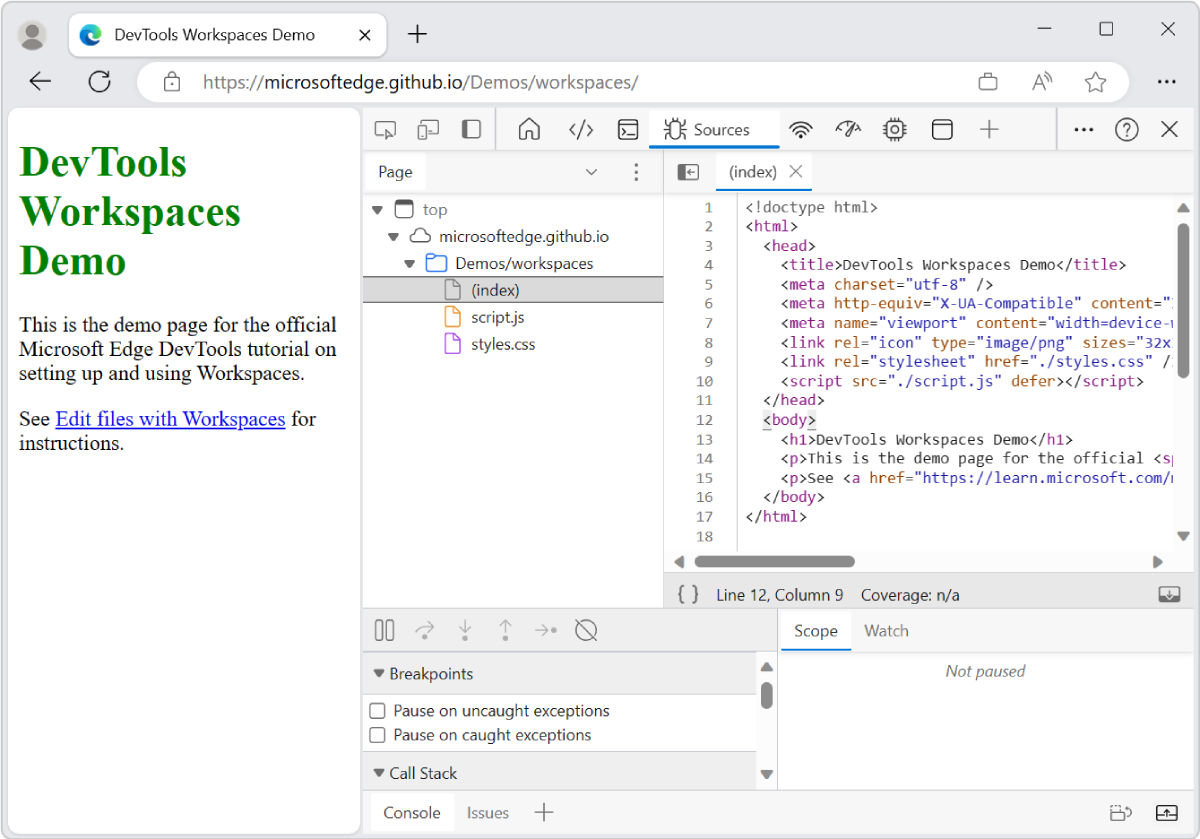
\includegraphics[width=0.7\linewidth]{assets/tools/edge-sources.png}
    \caption{Aba de código fonte - Microsoft Edge }
    \label{fig:enter-label}
\end{figure}
A ferramenta de codigo fonte auxilia os desenvolvedores a visualizar e interagir com os recursos de código subjacentes de uma página da web. Ele permite acessar arquivos como folhas de estilo (CSS), arquivos JavaScript e imagens, inspecionando seu conteúdo e caminho. Esta ferramenta serve como um centro de depuração de JavaScript e oferece a capacidade de editar CSS e JavaScript diretamente no navegador \cite{chrome}.

Uma das funcionalidades mais poderosas do painel Fontes é a depuração de JavaScript. Desenvolvedores podem definir pontos de interrupção em linhas específicas do código para pausar a execução, percorrer o código linha a linha (passo a passo) \cite{apple}, e inspecionar variáveis locais e globais, bem como a pilha de chamadas para entender o fluxo de execução e o estado da aplicação em tempo real. Para código minificado ou ofuscado, o painel suporta mapas de origem (source maps), permitindo que os desenvolvedores vejam e depurem o código original não minificado. Além disso, a funcionalidade de Workspaces permite que as alterações feitas no DevTools sejam salvas diretamente nos arquivos locais do sistema de arquivos do desenvolvedor, transformando o navegador em um editor de código \cite{edge}.

O painel Fontes também inclui recursos para otimização e automação do fluxo de trabalho. Os snippets são pequenos scripts JavaScript que podem ser criados, salvos e executados em qualquer página para realizar tarefas repetitivas ou testes rápidos. 

\section{Conta-gotas}
\begin{figure}[h!]
    \centering
    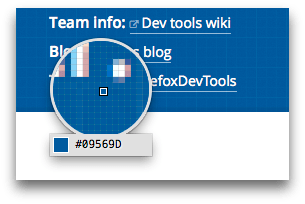
\includegraphics[width=0.7\linewidth]{assets/tools/firefox-eyedropper.png}
    \caption{ferramenta de conta-gotas - Mozilla Firefox }
    \label{fig:enter-label}
\end{figure}
A ferramenta conta-gotas (Eyedropper) nas ferramentas de desenvolvedor permite aos usuários selecionar cores diretamente de uma página web com precisão de pixel. Ela opera como uma lente de aumento, exibindo o valor da cor do pixel sob o cursor \cite{firefox}. Esta ferramenta pode ser utilizada para copiar a cor selecionada para a área de transferência ou para aplicar a cor amostrada diretamente em um valor de estilo CSS na visualização das Regras do Inspetor\cite{firefox}.

O conta-gotas está disponível nas ferramentas de desenvolvedor do Firefox. As ferramentas do Microsoft Edge e Google Chrome também incluem uma funcionalidade de conta-gotas dentro do seletor de cores, permitindo amostrar cores da página.
\newpage
\section{Console}
\begin{figure}[h!]
    \centering
    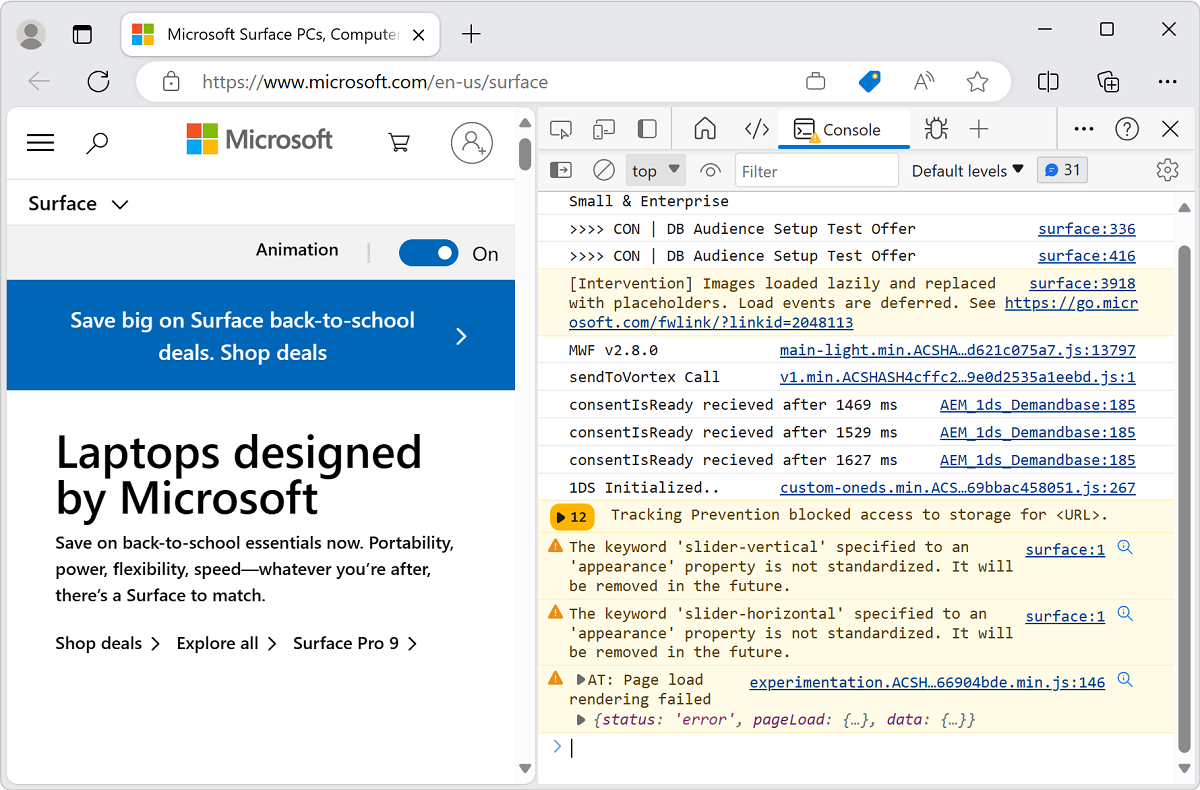
\includegraphics[width=0.7\linewidth]{assets/tools/edge-console.png}
    \caption{Aba de console - Microsoft Edge }
    \label{fig:enter-label}
\end{figure}
O Console é uma ferramenta fundamental em navegadores como Chrome, Edge, Firefox e Safari, funcionando como uma interface de linha de comando inteligente e rica e um sistema abrangente de registro para o desenvolvimento web. Seu principal propósito é auxiliar os desenvolvedores a depurar problemas em tempo real, visualizar mensagens registradas pelo código JavaScript e executar comandos JavaScript diretamente no ambiente do navegador\cite{chrome}. Ele permite interagir e manipular dinamicamente a página inspecionada, proporcionando um feedback imediato sobre quaisquer problemas no código.

Desenvolvedores frequentemente utilizam o Console para registrar mensagens, verificando se o JavaScript está sendo executado na ordem correta e inspecionando valores de variáveis em um determinado momento usando o método \texttt{console.log()} \cite{chrome}. Como um ambiente REPL (Read-Eval-Print Loop), o Console permite executar qualquer comando JavaScript para interagir com a página, modificar variáveis em tempo de execução ou testar novos trechos de código, tendo acesso total ao objeto window da página \cite{apple}.

A ferramenta Console também oferece funcionalidades adicionais, como a capacidade de usar console.time() e console.timeEnd() para medir o desempenho básico de trechos de código. Em alguns navegadores, como o Safari, o Console integra monitoramento de rede para analisar o tempo de requisições e respostas \cite{apple}. Ele facilita a depuração ao permitir que você clique em mensagens de erro para navegar diretamente para a linha ofensora no painel Fontes \cite{apple}. 

\section{Desempenho}
\begin{figure}[h!]
    \centering
    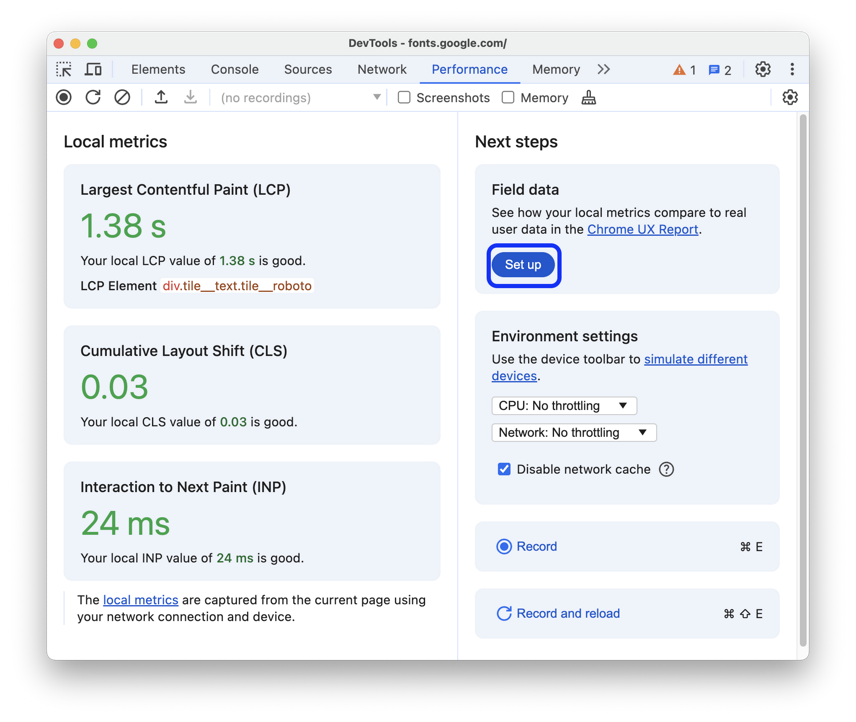
\includegraphics[width=0.7\linewidth]{assets/tools/chrome-performance.png}
    \caption{Aba de desempenho - Google Chrome }
    \label{fig:enter-label}
\end{figure}
A ferramenta de desempenho, também conhecida como Performance ou Profiler nos navegadores, é um conjunto de utilitários cruciais para analisar e otimizar a velocidade de carregamento e a responsividade de um site ou aplicação web . Ela permite gravar perfis de desempenho da CPU, memória, atividade de rede, execução de JavaScript, e operações de layout e renderização, ajudando a identificar gargalos e ineficiências\cite{chrome}.

Essas ferramentas permitem simular diversas condições de rede e CPU (como 3G lento ou CPU desacelerada) para entender como a página se comporta em diferentes ambientes de usuário . Além de métricas gerais de tempo, elas fornecem informações detalhadas sobre as Core Web Vitals, como o Largest Contentful Paint (LCP), Cumulative Layout Shift (CLS) e Interaction to Next Paint (INP), que medem o desempenho de carregamento, estabilidade visual e interatividade, respectivamente \cite{chrome}. 
\newpage
\section{Design responsivo}
\begin{figure}[h!]
    \centering
    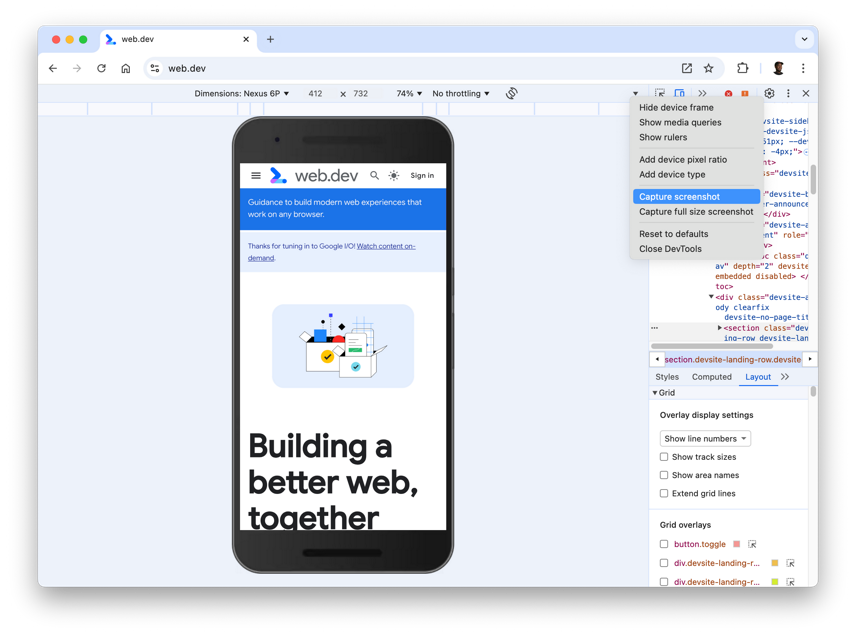
\includegraphics[width=0.7\linewidth]{assets/tools/chrome-device.png}
    \caption{Modo dispositivo - Google Chrome }
    \label{fig:enter-label}
\end{figure}
A ferramenta de Design Responsivo, também conhecida como Modo Dispositivo ou Emulação de Dispositivos em diferentes navegadores, é uma funcionalidade essencial nas ferramentas de desenvolvedor (DevTools) que permite simular como um website ou aplicação web se comporta e se parece em variados tamanhos de tela e tipos de dispositivo \cite{edge}. O objetivo é garantir que a interface do usuário se adapte de forma fluida e eficiente às características do dispositivo, como smartphones e tablets, utilizando técnicas como as CSS3 Media Queries \cite{firefox}. Isso é crucial para otimizar a experiência do usuário, permitindo aos desenvolvedores visualizar e depurar layouts sem a necessidade de múltiplos dispositivos físicos. Esta funcionalidade está amplamente disponivel nos navegadores citados nesse trabalho:
\begin{itemize}
    \item No Google Chrome, ela é acessível como "Modo dispositivo" (Device Mode), permitindo a simulação da viewport móvel, emulação de sensores e limitação da rede/CPU \cite{chrome}.
    \item No Microsoft Edge, a ferramenta "Device Emulation" oferece um "Responsive Viewport Mode" onde se pode ajustar dimensões, visualizar media queries, definir a proporção de pixels do dispositivo e controlar a rede/CPU \cite{edge}.
    \item No Mozilla Firefox, a funcionalidade é chamada de "Responsive Design Mode", que permite testar o site em diferentes dispositivos e tipos de rede, e pode até redimensionar a tela com base nas regras @media \cite{firefox}.
    \item No Safari Web Inspector, também há um "Responsive Design Mode" para testar media queries e estilos dinâmicos, garantindo uma boa aparência em qualquer tela \cite{apple}.
\end{itemize}

\section{Editor de estilos}
\begin{figure}[h!]
    \centering
    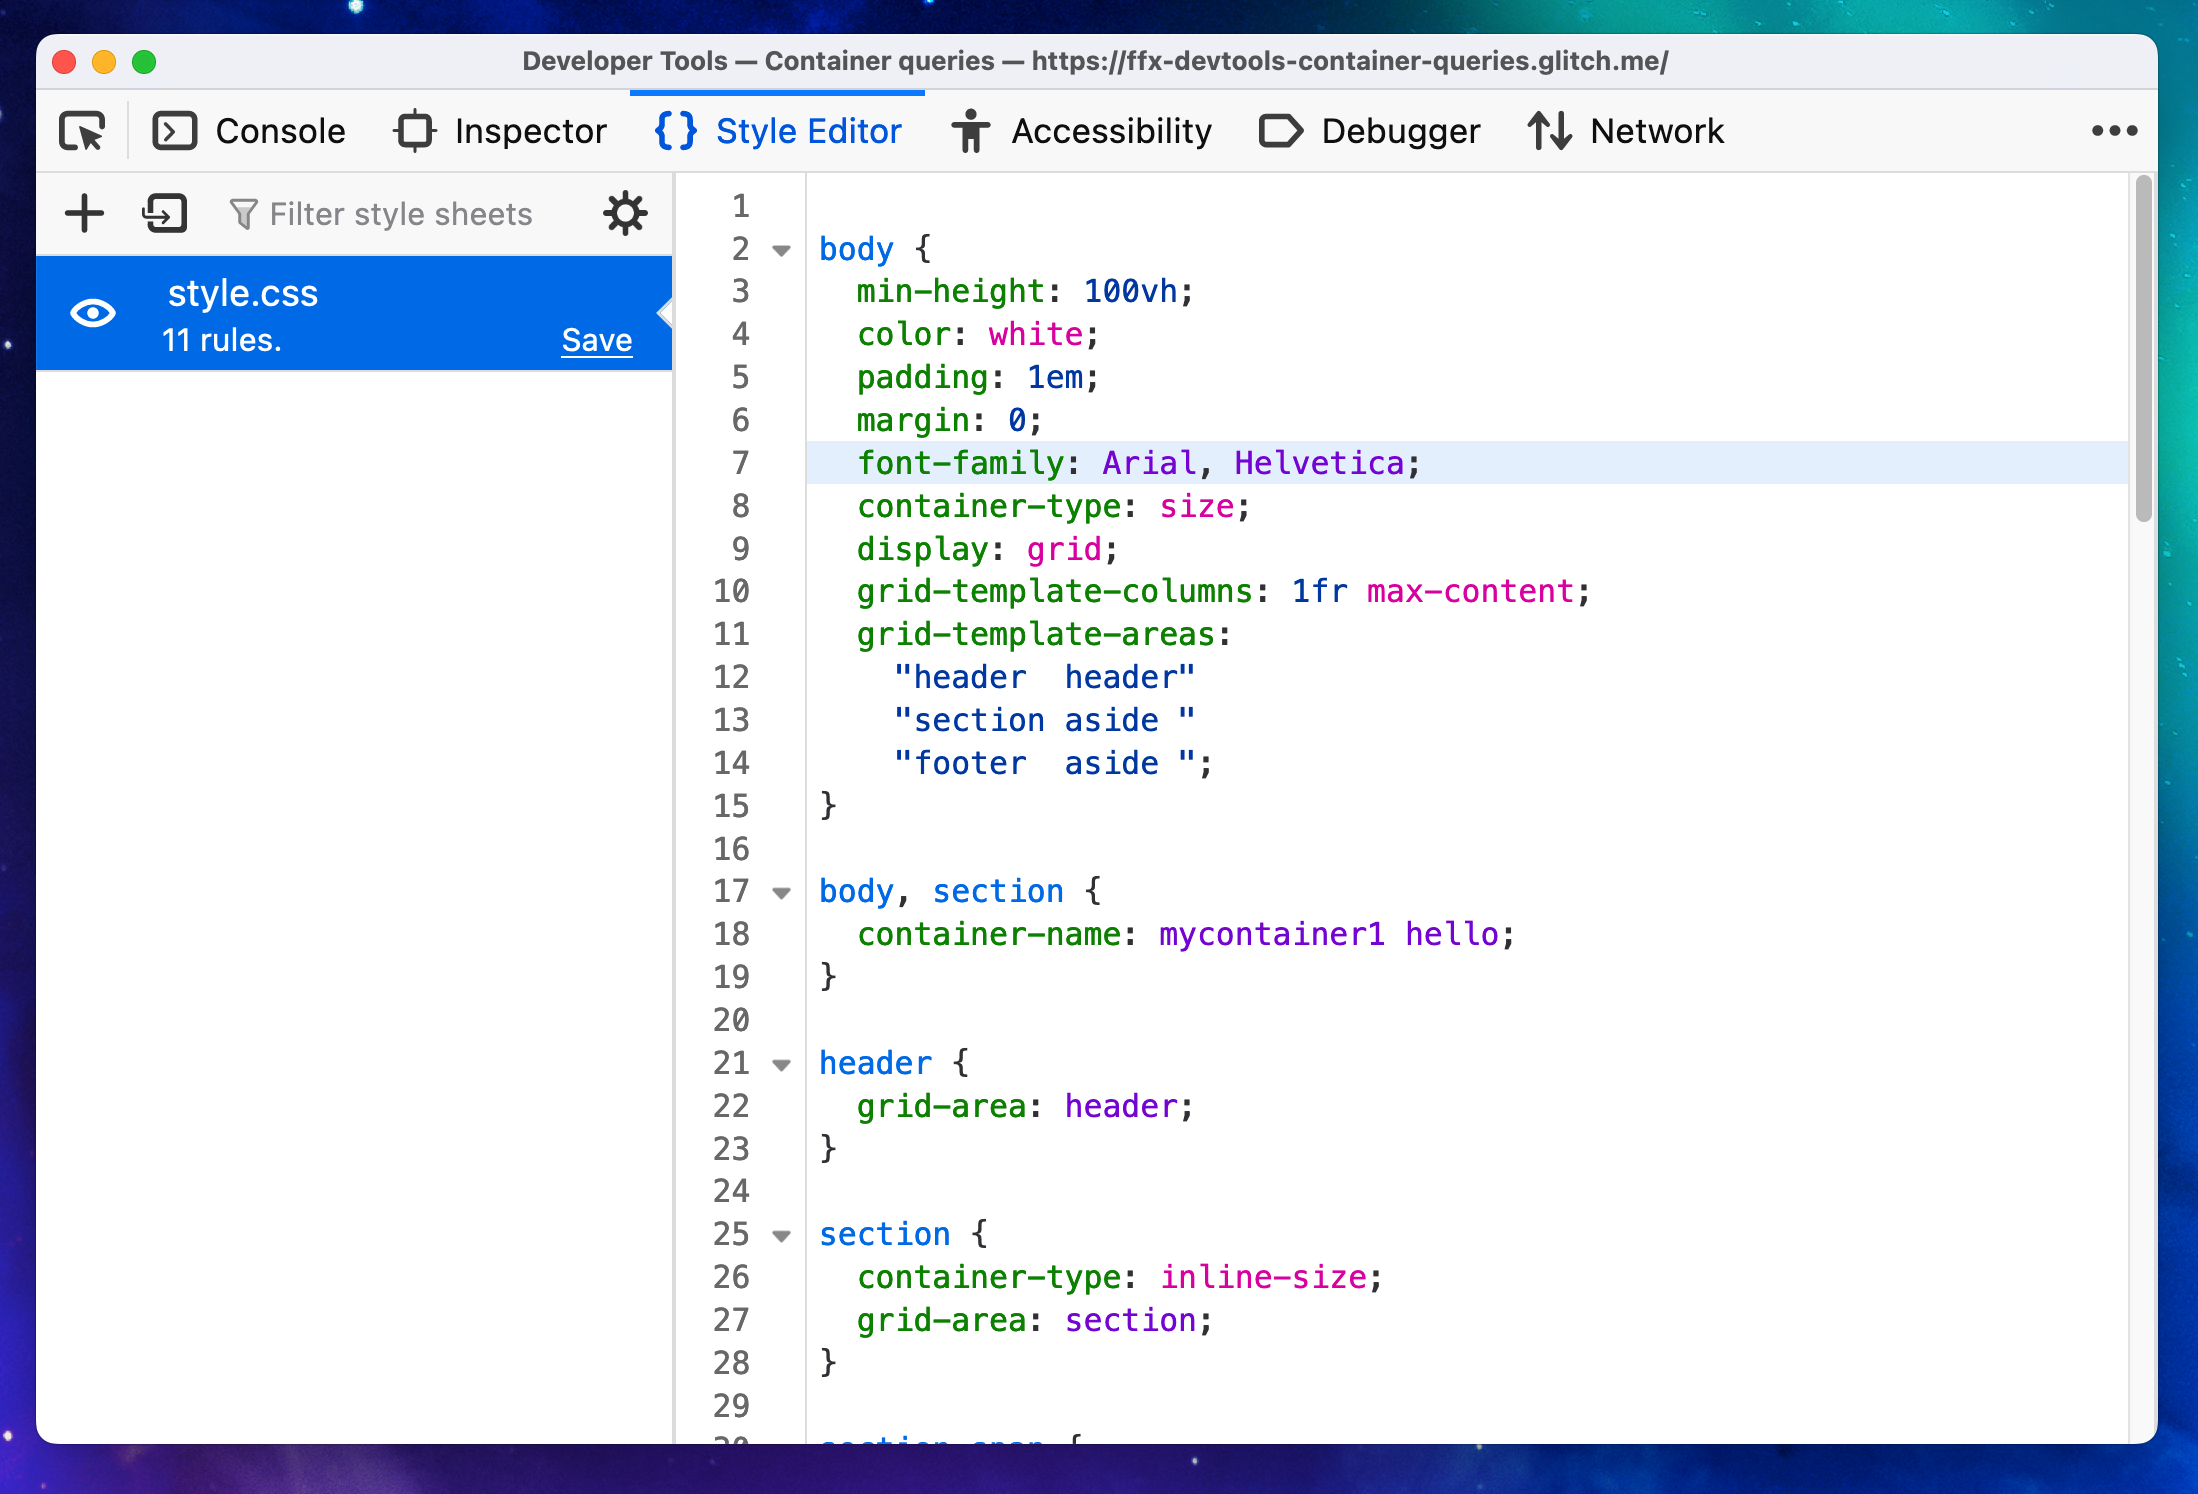
\includegraphics[width=0.7\linewidth]{assets/tools/firefox-style.png}
    \caption{Aba do editor de estilos - Mozilla Firefox }
    \label{fig:enter-label}
\end{figure}
O Editor de Estilos do Firefox DevTools é uma ferramenta que permite visualizar e modificar as folhas de estilo CSS associadas a uma página web. Ele oferece a capacidade de visualizar e editar todas as folhas de estilo, bem como criar novas do zero ou importar estilos existentes para aplicar à página \cite{firefox}. As alterações feitas no editor são aplicadas imediatamente na página, facilitando a experimentação e o teste de modificações. Além disso, você pode salvar as mudanças para o seu computador local.

O painel do Editor de Estilos inclui funcionalidades como numeração de linhas e destaque de sintaxe para melhor legibilidade do CSS, além de suporte a autocompletar. Ele também se destaca por sua capacidade de desminimizar automaticamente as folhas de estilo e oferecer suporte a "source maps", permitindo que você visualize e edite os arquivos CSS originais de pré-processadores como Sass, Less ou Stylus\cite{firefox}. 

O editor também exibe uma barra lateral de At-rules para regras como @media, @supports, @layer e @container, que é particularmente útil em conjunto com o Modo de Design Responsivo. Para abri-lo, basta selecionar o painel "Style Editor" nas Ferramentas do Desenvolvedor Web, acessível pelo submenu Browser Tools \cite{firefox}.

\section{Inspeção de elementos}

A ferramenta "Elementos" ou "Inspetor de Página", comumente conhecida como recurso "Inspecionar Elementos", é um componente fundamental das ferramentas de desenvolvimento integradas nos navegadores Chrome, Edge, Firefox e Safari. Seu objetivo principal é permitir que desenvolvedores web inspecionem e manipulem o Modelo de Objeto de Documento (DOM) e as Folhas de Estilo em Cascata (CSS) de uma página web renderizada em tempo real \cite{chrome}. Esta ferramenta oferece uma visualização em tempo real da estrutura da página, possibilitando edições rápidas e o diagnóstico de problemas \cite{chrome}. Ao ser ativada, passar o mouse sobre os elementos na página exibe uma sobreposição de informações e destaque da grade, mostrando detalhes como dimensões, cor, configurações de fonte e margens/preenchimento.

\begin{figure}[h!]
    \centering
    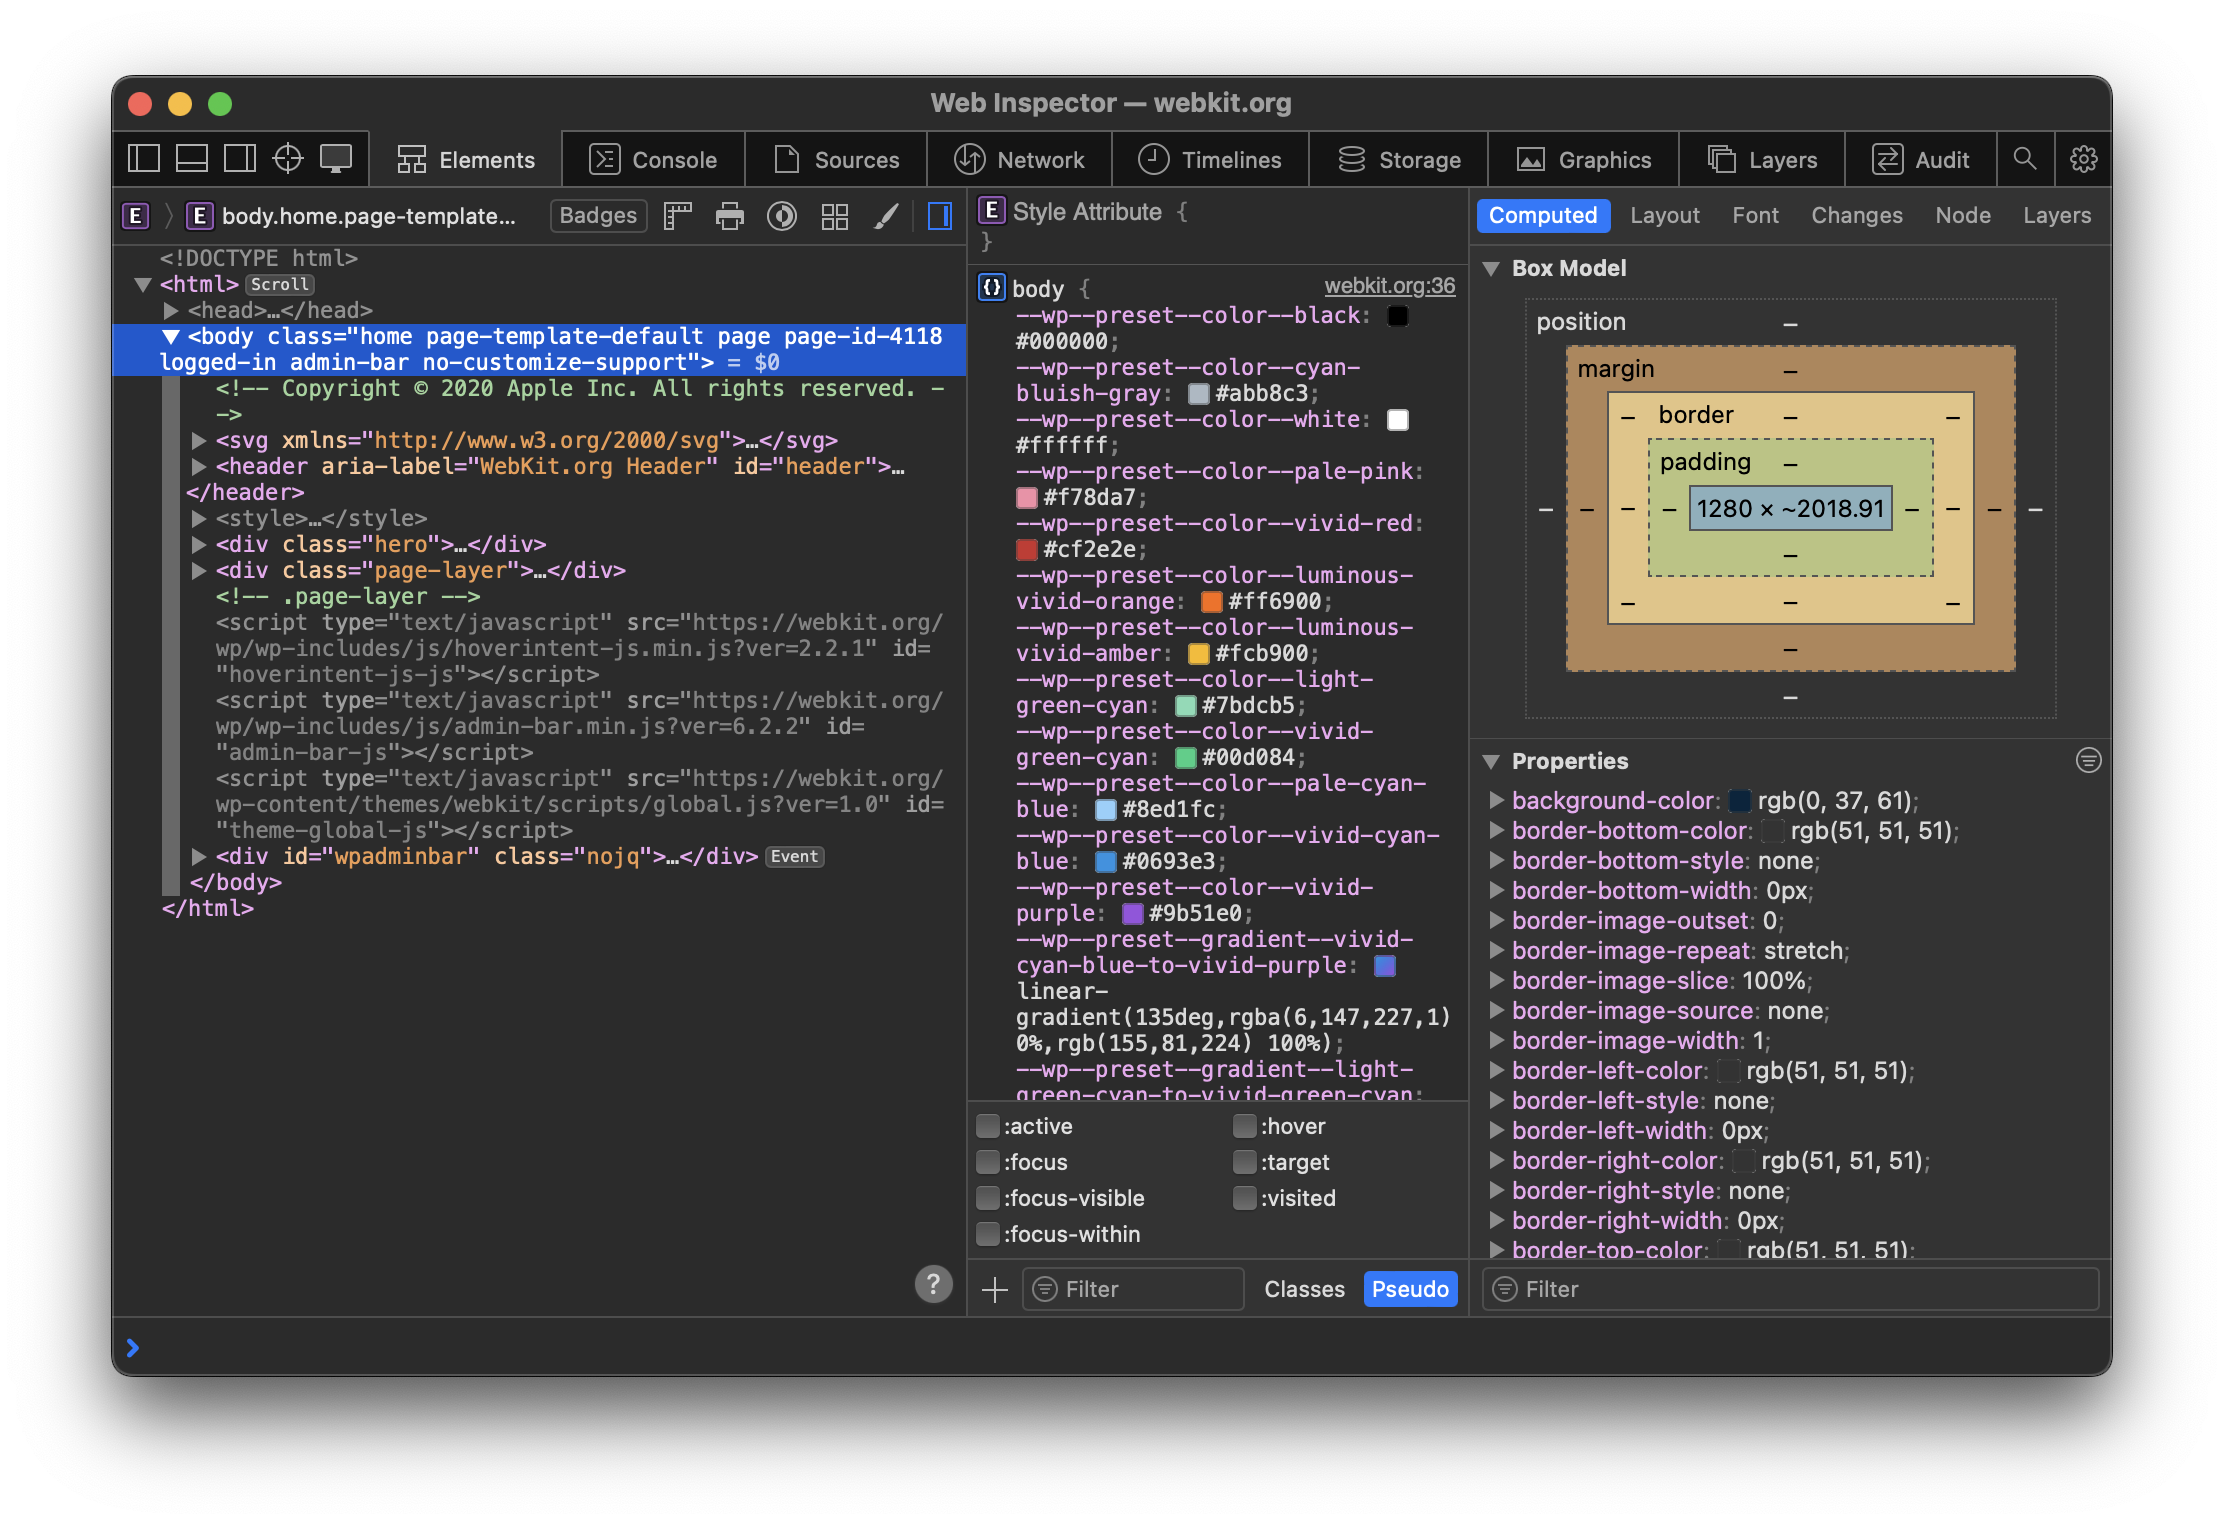
\includegraphics[width=0.7\linewidth]{assets/tools/safari-elements.png}
    \caption{Aba do inspeção de elementos - Safari }
    \label{fig:enter-label}
\end{figure}

Dentro da ferramenta Elementos, os desenvolvedores podem realizar uma ampla gama de ações. Ela apresenta o DOM como uma árvore editável, onde nós individuais podem ser selecionados, reordenados por arrasto ou editados diretamente (por exemplo, tag, atributo, texto). O painel "Estilos" associado permite uma visualização e depuração abrangente das regras CSS, incluindo estilos computados, e a capacidade de adicionar novas declarações ou aplicar classes, com estilos inválidos ou substituídos claramente indicados \cite{edge}. Além disso, oferece recursos para inspecionar listeners de eventos, definir pontos de interrupção do DOM (por exemplo, para modificações de subárvore ou remoção de nós), e examinar as propriedades e informações de acessibilidade de um elemento, como marcadores ARIA e problemas de contraste \cite{apple}. Opções específicas de layout para CSS Grid e Flexbox também estão disponíveis. A ferramenta pode até mesmo forçar estados como :hover ou :active para auxiliar na depuração de estilo e comportamento \cite{edge}.

É considerada indispensável para o desenvolvimento front-end, oferecendo insights que vão além de meras mudanças visuais, permitindo que os desenvolvedores compreendam profundamente como a estrutura, os estilos e os comportamentos interativos de uma página são renderizados e interagem \cite{chrome}. A disponibilidade consistente desses recursos em diferentes navegadores ressalta seu papel crítico na construção e manutenção de aplicações web de alta qualidade, desempenho e acessibilidade.
\section{Inspetor de memória}
O Inspetor de Memória e o painel Memória, presentes nas ferramentas de desenvolvedor do Chrome e Edge, auxiliam a analisar e otimizar o uso de memória em aplicações web. Ele suporta diversos tipos de perfil, como instantâneos de heap (para uso imediato da memória por objeto) e instrumentação de alocação na linha do tempo (para rastrear alocações ao longo do tempo e localizar vazamentos) \cite{edge}.

O Inspetor de Memória é projetado para inspecionar a memória bruta de estruturas de dados como ArrayBuffer, TypedArray e DataView em JavaScript, bem como WebAssembly.Memory em aplicações C++ \cite{chrome}. Essa ferramenta organiza o conteúdo da memória para facilitar a navegação, permite a visualização de valores ASCII ao lado dos bytes, e oferece a capacidade de selecionar diferentes configurações de endianness, tornando-a altamente eficaz para depuração de memória de baixo nível \cite{chrome}. Essa ferramenta contribui significativamente para a compreensão e resolução de problemas de desempenho relacionados ao consumo de memória.

\section{Auditoria}
As ferramentas de auditoria auxiliam os desenvolvedores web a analisar e otimizar a qualidade, o desempenho e a acessibilidade de seus sites. Embora possam ter nomes e ênfases ligeiramente diferentes dependendo do navegador, o objetivo principal é fornecer insights acionáveis para melhorar a experiência do usuário e a conformidade com as melhores práticas da web
.
No Chrome DevTools, o Lighthouse é uma ferramenta de auditoria abrangente que gera um relatório detalhado sobre o desempenho, acessibilidade, melhores práticas e SEO de um site \cite{chrome}. Ele cria uma linha de base de desempenho e oferece dicas práticas sobre quais mudanças terão o maior impacto na velocidade de carregamento da página. O relatório do Lighthouse inclui métricas como First Contentful Paint e Time To Interactive, além de identificar oportunidades para otimização, como ativação de compressão de texto, redimensionamento de imagens e eliminação de recursos que bloqueiam a renderização \cite{chrome}. Em navegadores como o Safari Web Inspector, existe uma guia dedicada a Auditorias (Audit Tab), que permite executar coleções de testes automatizados para verificar a estrutura do DOM, atributos de acessibilidade ausentes, e conformidade com regras de design \cite{apple}.

Essas auditorias podem resultar em diferentes níveis de falha, como "Pass" (aprovado), "Warning" (aviso), "Failed" (falhou) ou "Error" (erro), e fornecem informações detalhadas sobre os recursos afetados. A ferramenta também oferece a capacidade de criar e modificar auditorias personalizadas, tornando-a uma ferramenta flexível para garantir que as páginas sigam diretrizes e especificações modernas.

\section{Medidas da página}
a

\section{Memória}
a

\section{Mídia}
a

\section{Monitor de desempenho}
a

\section{Monitor de protocolos}
a

\section{Network}
A ferramenta de Rede (Network) nos navegadores web é uma funcionalidade crucial para desenvolvedores, integrada diretamente nas ferramentas de desenvolvedor (DevTools), que permite analisar o carregamento de páginas e inspecionar recursos de rede. Ela é essencial para garantir que os recursos da sua página web sejam baixados conforme o esperado e que as solicitações às APIs do lado do servidor sejam enviadas corretamente \cite{edge}. Geralmente, pode ser acessada através de atalhos de teclado como Ctrl + Shift + J (Windows, Linux) ou Command + Option + J (macOS), que abrem diretamente o console, ou através do menu DevTools, navegando para a aba "Network"
.
No painel de Rede, é possivel encontrar uma visão geral detalhada das atividades de rede, incluindo uma barra de ferramentas para personalizar e filtrar solicitações, um gráfico de visão geral mostrando o tráfego de rede ao longo do tempo, e o log de rede que lista as solicitações individuais \cite{apple}. Cada solicitação no log exibe informações como status HTTP, tipo de recurso, iniciador, tamanho, duração e um gráfico em cascata (Waterfall) que detalha as diferentes fases da solicitação. As ferramentas também permitem filtrar e classificar solicitações por propriedades como domínio ou tipo, e pesquisar cabeçalhos e respostas HTTP \cite{chrome}. Essa capacidade de manipulação e observação é fundamental para otimizar o desempenho, identificar gargalos e depurar problemas relacionados à rede nas aplicações web.

\section{Origem rápida}
a

\section{Problemas}
a

\section{Recursos para desenvolvedores}
a

\section{Régua}
a

\section{Renderizador}
a

\section{Segurança}
a

\section{Sensores}
a

\section{Timeline}
a

\section{Visão geral do CSS}
a

\section{Visualizador de propriedade DOM}
a

\section{WebAudio}
a

\section{WebAuthn}
a

\section{WebDriver}
a

\begin{table}[htbp!]
\centering
\begin{tabularx}{\textwidth}{|p{4cm}|X|p{3cm}|X|X|}
\hline
\multirow{2}{*}{Funcionalidades} & \multicolumn{4}{c|}{Ferramentas} \\ \cline{2-5}
 & Google Chrome & Firefox & Edge & Safari \\ \hline
Inspeção de elementos   & Elements (Elementos) & Page Inspector (Inspetor de Página) & Elements (Elementos) & Elements (Elementos) \\ \hline
Console                 & Console & Web Console (Console da Web) & Console & Console \\ \hline
Depurador JavaScript    & Sources (Origens)  & JavaScript Debugger (Depurador JavaScript) & Sources (Origens) & Sources (Fontes) \\ \hline
Monitoramento de Rede   & Network (Rede) & Network Monitor (Monitor de Rede) & Network (Rede) & Network (Rede) \\ \hline
Análise de desempenho & Performance (Desempenho) & Performance Panel (Painel de desempenho) & Timeline (Linha do tempo) & \\ \hline
Análise de Memória & Memory (Memória)& Memory Tool (Ferramenta de Memória) & Timeline (Linha do tempo) & \\ \hline
Armazenamento de Aplicação & Application (Aplicativo) & Storage Inspector (Inspetor de Armazenamento) & Application (Aplicativo) & Storage (Armazenamento) \\ \hline
Edição e Manipulação de estilos & Elements (Elementos) & Style Editor (Editor de estilos) & Elements (Elementos) & Elements (Elementos) \\ \hline
Inspeção de segurançã & Security (Segurança) & & Security (Segurança) & Network (Rede) \\ \hline
Emulação de dispositivos / Responsividade & Device Mode (Modo Dispositivo) & Responsive Design Mode (Modo de Design Responsivo) & Device Mode (Modo dispositivo) & Responsive Design Mode (Modo de Design Responsivo) \\ \hline
Inspeção e edição de animações & Animations (Animações) & Page inspector (Inspetor de Página) & Animations (Animações) & Graphics (Graficos) \\ \hline
Análise de Acessibilidade & Lighthouse & Accessibillity Inspector (Inspetor de Acessibilidade) & Lighthouse & Audit (Auditoria) \\ \hline
Auditoria de qualidade e desempenho & Lighthouse &  & Lighthouse & Audit (Auditoria) \\ \hline
Cobertura de código/rastreamento & Coverage (Cobertura) &   & Coverage (Cobertura) &  \\ \hline
Gravar/reproduzir fluxo do usuário & Recorder (Gravador) &  & Recorder (Gravador) &  \\ \hline
\end{tabularx}
\end{table}
\include{src/textuais/resultados}

\postextual
% INSERE ELEMENTOS PÓS-TEXTUAIS
% REFERÊNCIAS------------------------------------------------------------------

% Carrega o arquivo "base-referencias.bib" e extrai automaticamente as referências citadas

\bibliography{referencias}{}
\bibliographystyle{abntex2-alf} % Define o estilo ABNT para formatar a lista de referências

% OBSERVAÇÕES------------------------------------------------------------------
% Este arquivo não precisa ser alterado.
        % Referências

\end{document}
